\label{cap:exper}
Nesta seção serão mostrados os resultados experimentais do capítulo \ref{cap:desen}. As saídas de alguns resultados podem ser encontradas no arquivo Jupyter-notebook no \href{https://github.com/joaomh/study_boosting_optuna_USP_undergraduate_thesis}{GitHub}. As análises consistem em alterar os hiperparâmetros, conforme explicado no capítulo \ref{cap:desen}, depois aplicar o Optuna para os 3 modelos, com o tempo máximo de execução de trinta minutos para cada um.
\section{Resultados de Conjunto de dados de Diabetes}
\begin{table}[H]
\centering
\begin{tabular}{|c|c|c|c|}
\hline
	& \textbf{XGBoost} &\textbf{CatBoost} & \textbf{LightGBM} \\
\hline
\textbf{AUC}	&0.93639	& 0.89655	& 0.92066 \\
\hline
\textbf{logloss}	& 1.69072 & 2.65684	& 2.29456 \\
\hline
\textbf{KS}	& 0.87278	& 0.79311	& 0.84131 \\
\hline
\textbf{tempo (s)}	& 0.17799 &	 1.78698 &	0.08261 \\
\hline
\end{tabular}
\caption{Resultado do XGBoost, CatBoost e LGBM com os hiperparâmetros \textit{Default} no conjunto de dados de diabetes.}\label{res:dia:1}
\end{table}

\begin{table}[H]
\label{res:dia:2}
\centering
\begin{tabular}{|c|c|c|c|}
\hline
	& \textbf{XGBoost} &\textbf{CatBoost} & \textbf{LightGBM} \\
\hline
\textbf{AUC}	& 0.92598	& 0.89428	& 0.89406\\
\hline
\textbf{logloss}	& 2.17379	& 3.13992	& 2.89838\\
\hline
\textbf{KS}	& 0.85195	& 0.78856	0& 0.78812 \\
\hline
\textbf{tempo (s)}	& 0.10825	& 1.05492	& 0.09304 \\
\hline
\end{tabular}
\caption{Resultado do XGBoost, CatBoost e LGBM com os hiperparâmetros $LR=0.1$, $MD=3$, $Reg_L=0.01$ no conjunto de dados de diabetes.}
\end{table}

\begin{table}[H]
\label{res:dia:3}
\centering
\begin{tabular}{|c|c|c|c|}
\hline
	& \textbf{XGBoost} &\textbf{CatBoost} & \textbf{LightGBM} \\
\hline
\textbf{AUC}	& 0.92598	&0.90448	&0.92598\\
\hline
\textbf{logloss}	& 2.17379	&2.41531	&2.17379\\
\hline
\textbf{KS}	& 0.85195	& 0.80895 &	0.85195 \\
\hline
\textbf{tempo (s)}	& 0.11743&	1.00966&	0.08180 \\
\hline
\end{tabular}
\caption{Resultado do XGBoost, CatBoost e LGBM com os hiperparâmetros $LR=0.3$, $MD=3$, $Reg_L=0.01$ no conjunto de dados de diabetes.}
\end{table}

\begin{table}[H]
\label{res:dia:4}
\centering
\begin{tabular}{|c|c|c|c|}
\hline
	& \textbf{XGBoost} &\textbf{CatBoost} & \textbf{LightGBM} \\
\hline
\textbf{AUC}	& 0.93107&	0.91534	&0.92066\\
\hline
\textbf{logloss}	& 1.81149	&2.41532	&2.29456\\
\hline
\textbf{KS}	& 0.86215	& 0.83067	& 0.84131\\
\hline
\textbf{tempo (s)}	& 0.12579	&1.82060	&0.11067\\
\hline
\end{tabular}
\caption{Resultado do XGBoost, CatBoost e LGBM com os hiperparâmetros $LR=0.1$, $MD=6$, $Reg_L=0.01$ no conjunto de dados de diabetes.}
\end{table}

\begin{table}[H]
\label{res:dia:5}
\centering
\begin{tabular}{|c|c|c|c|}
\hline
	& \textbf{XGBoost} &\textbf{CatBoost} & \textbf{LightGBM} \\
\hline
\textbf{AUC}	& 0.89406	&0.89428	&0.89406\\
\hline
\textbf{logloss}	& 2.89838	&3.13992&	2.89838\\
\hline
\textbf{KS}	& 0.78812&	0.78856 &	0.78812\\
\hline
\textbf{tempo (s)}	& 0.09512	&1.38364	&0.08838\\
\hline
\end{tabular}
\caption{Resultado do XGBoost, CatBoost e LGBM com os hiperparâmetros $LR=0.1$, $MD=3$, $Reg_L=0.05$ no conjunto de dados de diabetes.}
\end{table}

\begin{table}[H]
\label{res:dia:6}
\centering
\begin{tabular}{|c|c|c|c|}
\hline
	& \textbf{XGBoost} &\textbf{CatBoost} & \textbf{LightGBM} \\
\hline
\textbf{AUC}	& 0.93107&	0.89927	&0.92598\\
\hline
\textbf{logloss}	& 1.81149	&2.65685	&2.17379\\
\hline
\textbf{KS}	& 0.86215	&0.79854	&0.85195 \\
\hline
\textbf{tempo (s)}	& 0.13494	&2.58085	&0.09262 \\
\hline
\end{tabular}
\caption{Resultado do XGBoost, CatBoost e LGBM com os hiperparâmetros $LR=0.3$, $MD=6$, $Reg_L=0.01$ no conjunto de dados de diabetes.}
\end{table}

\begin{table}[H]
\label{res:dia:7}
\centering
\begin{tabular}{|c|c|c|c|}
\hline
	& \textbf{XGBoost} &\textbf{CatBoost} & \textbf{LightGBM} \\
\hline
\textbf{AUC}	& 0.92836	&0.90470	&0.92598\\
\hline
\textbf{logloss}	& 1.81148&	2.65685&	2.17379\\
\hline
\textbf{KS}	&0.85672&	0.80940	&0.85195\\
\hline
\textbf{tempo (s)}	& 0.13301	&1.81456	&0.10295 \\
\hline
\end{tabular}
\caption{Resultado do XGBoost, CatBoost e LGBM com os hiperparâmetros $LR=0.3$, $MD=6$, $Reg_L=0.05$ no conjunto de dados de diabetes.}
\end{table}

\begin{table}[H]
\label{res:dia:8}
\centering
\begin{tabular}{|c|c|c|c|}
\hline
	& \textbf{XGBoost} &\textbf{CatBoost} & \textbf{LightGBM} \\
\hline
\textbf{AUC}	& 0.92598&	0.90492&	0.92598\\
\hline
\textbf{logloss}	& 2.17379&	2.89839	&2.17379\\
\hline
\textbf{KS}	& 0.85195	&0.80984	&0.85195 \\
\hline
\textbf{tempo (s)}	& 0.10512&	0.97739	&0.09690 \\
\hline
\end{tabular}
\caption{Resultado do XGBoost, CatBoost e LGBM com os hiperparâmetros $LR=0.3$, $MD=3$, $Reg_L=0.05$ no conjunto de dados de diabetes.}
\end{table}
\subsection{Optuna no Conjunto de dados de Diabetes}
No final da execução, o Optuna nos retorna a quantidade de \textit{trials} e qual foi a que obteve a melhor performance. Abaixo temos os códigos com as melhores saídas do Optuna de cada modelo.
\begin{codigo}[caption={Resultado do Optuna no conjunto de dados de Diabetes.}, label={codigo:res:op:dia}, language=Python, breaklines=true]
XGBoost_model = train(X_train, y_train, X_test, y_test, balanced='balanced', method='XGBoost')
Trial 5143 finished with value: 0.9734596631205674 and parameters: {'learning_rate': 0.08503540937695053, 'max_depth': 16, 'min_child_weight': 1, 'gamma': 0.3765138366132899, 'alpha': 0.00011157064804299481, 'lambda': 0.06609519167136822, 'colsample_bytree': 0.7351361006258642}. Best is trial 5052 with value: 0.9759530141843972.
...
Trial 5052 finished with value: 0.9759530141843972 and parameters: {'learning_rate': 0.09999081729983263, 'max_depth': 15, 'min_child_weight': 1, 'gamma': 0.7591251036860868, 'alpha': 0.00010662969781278809, 'lambda': 0.06239587908284276, 'colsample_bytree': 0.7655930247173538}. Best is trial 5052 with value: 0.9759530141843972.
XGBoost - Optimization using optuna
auc:0.9759530141843972 , log_loss:0.17300349809156104 , ks:0.8782136524822696

CatBoost_model = train(X_train_cat, y_train_cat, X_test_cat, y_test_cat, balanced='balanced', method='CATBoost')
Trial 230 finished with value: 0.9786125886524822 and parameters: {'learning_rate': 0.008066790947749524, 'depth': 10, 'max_bin': 282, 'min_data_in_leaf': 48, 'l2_leaf_reg': 2.120609777416555, 'random_strength': 1.9674219542672667e-06, 'bagging_temperature': 6.752333264637867, 'od_type': 'Iter', 'od_wait': 16}. Best is trial 160 with value: 0.9811059397163121.
...
Trial 160 finished with value: 0.9811059397163121 and parameters: {'learning_rate': 0.005585552379158199, 'depth': 10, 'max_bin': 316, 'min_data_in_leaf': 11, 'l2_leaf_reg': 1.1081451827078879, 'random_strength': 7.466692400471057e-07, 'bagging_temperature': 9.443675875030443, 'od_type': 'IncToDec', 'od_wait': 17}. Best is trial 160 with value: 0.9811059397163121.
CATBoost - Optimization using optuna
auc:0.9811059397163121 , log_loss:0.17088682855569354 , ks:0.8779920212765957

LGBM_model = train(X_train, y_train, X_test, y_test, balanced='balanced', method='LGBM')
Trial 4540 finished with value: 0.9765625 and parameters: {'learning_rate': 0.07003556517783399, 'num_leaves': 191, 'lambda_l1': 3.2225284078443206e-06, 'lambda_l2': 4.1456610637867624e-08, 'min_data_in_leaf': 11, 'max_depth': 55, 'feature_fraction': 0.9234036984685567, 'bagging_fraction': 0.630684594822488, 'bagging_freq': 6}. Best is trial 1283 with value: 0.9816626773049646.
...
Trial 1283 finished with value: 0.9806626773049646 and parameters: {'learning_rate': 0.08425779644832665, 'num_leaves': 205, 'lambda_l1': 2.7481689793447196e-06, 'lambda_l2': 4.307867154100011e-08, 'min_data_in_leaf': 9, 'max_depth': 63, 'feature_fraction': 0.9232766751662997, 'bagging_fraction': 0.9517850099076617, 'bagging_freq': 6}. Best is trial 1283 with value: 0.9806626773049646.
LGBM - Optimization using optuna
auc:0.9816626773049646 , log_loss:0.1859868135509998 , ks:0.8832003546099291

\end{codigo}

\begin{table}[H]
\centering
\begin{tabular}{|c|c|c|c|}
\hline
	& \textbf{XGBoost} &\textbf{CatBoost} & \textbf{LightGBM} \\
\hline
\textbf{AUC}	& 0.97595	&0.981106	&0.98166\\
\hline
\textbf{logloss}	& 0.17300&	0.17327	&0.18599\\
\hline
\textbf{KS}	& 0.87821&	0.87799&	0.88320\\
\hline
\end{tabular}
\caption{Resultado do XGBoost, CatBoost e LGBM com os hiperparâmetros otimizados pelo Optuna no conjunto de dados de diabetes.}\label{res:dia:op}
\end{table}


\subsection{Resultados do estudo do Optuna no conjunto de dados de Diabetes utilizando o XGBoost.}
A primeira coisa é analisar todos os treinos e os valores encontrados para cada interação do Optuna para cada modelo.
\begin{figure}[H]
 \caption{Valores do estudo do XGBoost no conjunto de dados de Diabetes pelo Optuna.}
 \label{fig:op:dia:trials:xgb}
 \centering
 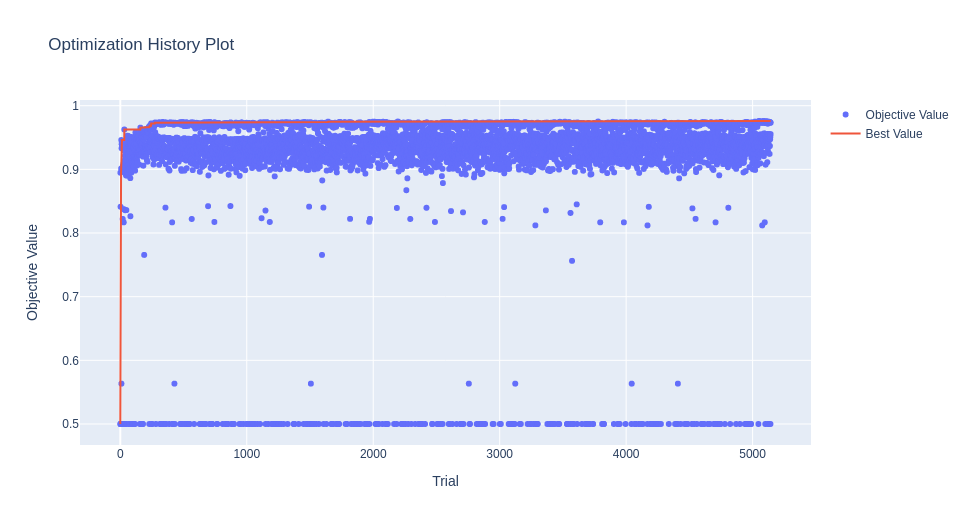
\includegraphics[scale=0.4]{images/optuna_xgboost_dia.png}
\end{figure}
A partir do estudo de otimização do Optuna foi possível identificar quais os hiperparâmetros que possuem o maior impacto no tuning do Optuna.
\begin{figure}[H]
 \caption{Hiperparâmetros do XGBoost com maior importância no Optuna no dados de Diabetes.}
 \label{fig:op:dia:impo:xgb}
 \centering
 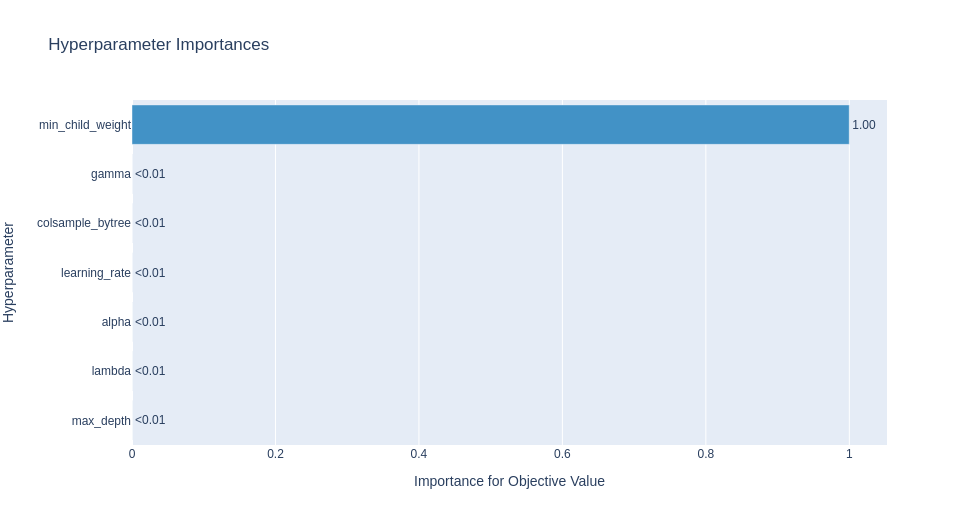
\includegraphics[scale=0.4]{images/importance_xgboost_dia.png}
\end{figure}
Ou seja, podemos concluir que ao longo do estudo do Optuna o hiperparâmetro com maior importância no resultado final foi o \textit{min\_child\_weight}.
% \begin{figure}[H]
%  \caption{Hiperparâmetros \textit{min\_child\_weight} do XGBoost no estudo do Optuna no conjunto de dados de Diabetes.}.
%  \label{fig:op:dia:min:xgb}
%  \centering
%  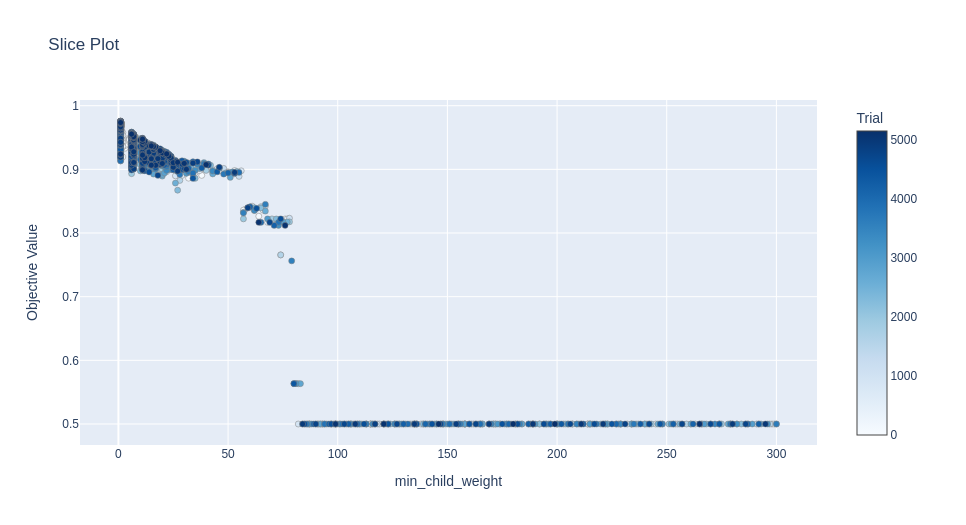
\includegraphics[scale=0.4]{images/optuna_xgboost_min_dia.png}
% \end{figure}

\subsection{Resultados do estudo do Optuna no conjunto de dados de Diabetes utilizando o CatBoost.}
\begin{figure}[H]
 \caption{Valores do estudo do CatBoost no conjunto de dados de Diabetes pelo Optuna.}
 \label{fig:op:dia:trials:cat}
 \centering
 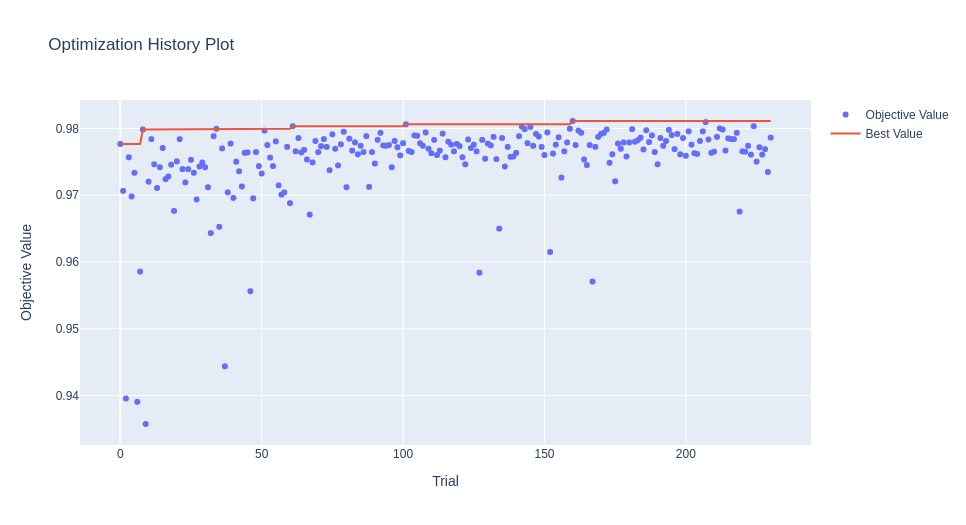
\includegraphics[scale=0.4]{images/optuna_catboost_dia.png}
\end{figure}
A partir do estudo de otimização do Optuna foi possível identificar quais os hiperparâmetros que possuem o maior impacto no tuning do Optuna.
\begin{figure}[H]
 \caption{Hiperparâmetros do XGBoost com maior importância no Optuna no dados de Diabetes.}
 \label{fig:op:dia:impo:cat}
 \centering
 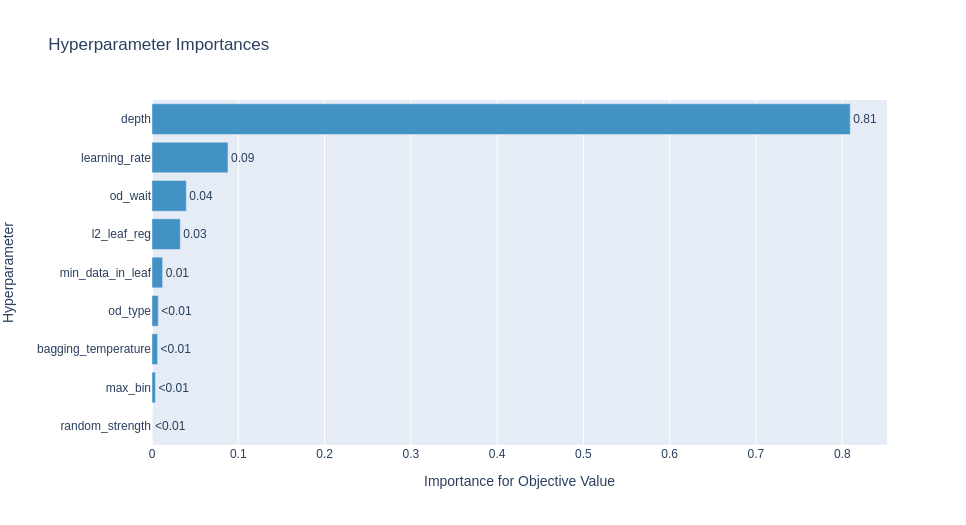
\includegraphics[scale=0.4]{images/importance_catboost_dia.png}
\end{figure}
Ou seja, podemos concluir que ao longo do estudo do Optuna o hiperparâmetro com maior importância no resultado final foram o \textit{depth} e o \textit{learning\_rate}.
% \begin{figure}[H]
%  \caption{Hiperparâmetros \textit{depth} do CatBoost no estudo do Optuna no conjunto de dados de Diabetes.}.
%  \label{fig:op:dia:dep:cat}
%  \centering
%  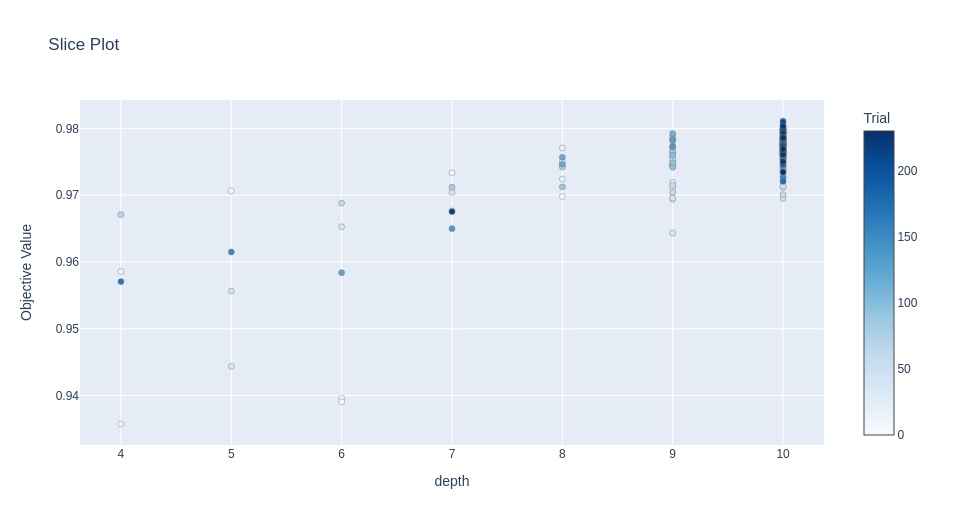
\includegraphics[scale=0.4]{images/optuna_cat_depth_dia.png}
% \end{figure}
% \begin{figure}[H]
%  \caption{Hiperparâmetros \textit{learning\_rate} do CatBoost no estudo do Optuna no conjunto de dados de Diabetes.}.
%  \label{fig:op:dia:dep:cat}
%  \centering
%  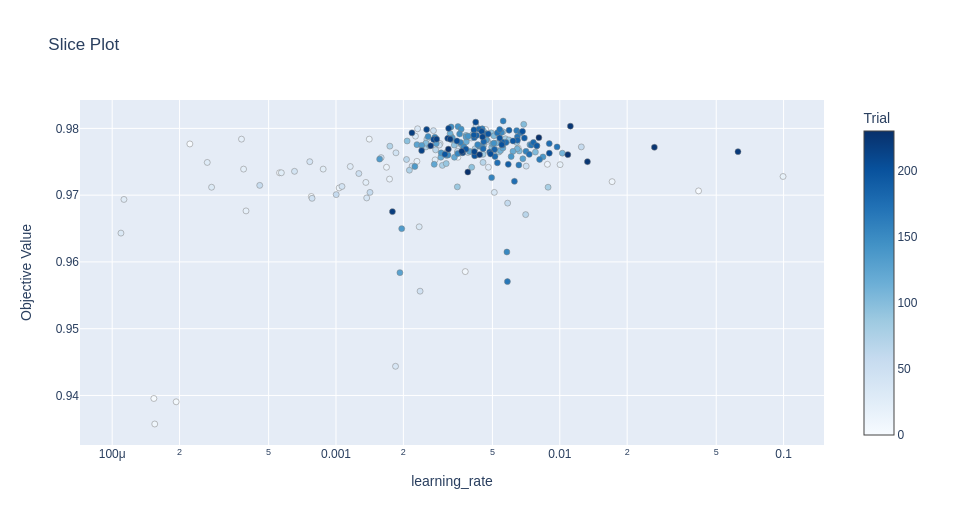
\includegraphics[scale=0.4]{images/optuna_cat_learnig_dia.png}
% \end{figure}

\subsection{Resultados do estudo do Optuna no conjunto de dados de Diabetes utilizando o LightGBM.}
\begin{figure}[H]
 \caption{Valores do estudo do LightGBM no conjunto de dados de Diabetes pelo Optuna.}.
 \label{fig:op:dia:trials:lgbm}
 \centering
 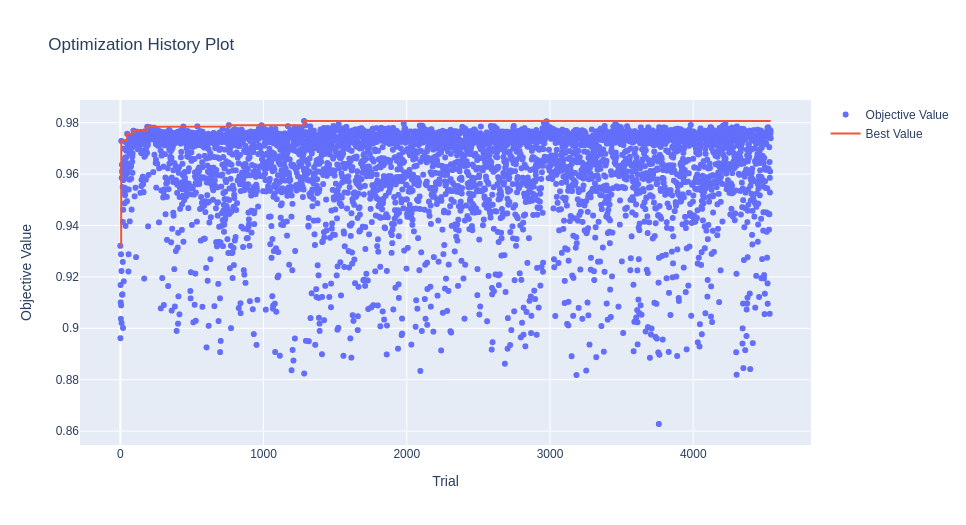
\includegraphics[scale=0.4]{images/optuna_lgbm_dia.png}
\end{figure}
A partir do estudo de otimização do Optuna foi possível identificar quais os hiperparâmetros que possuem o maior impacto no tuning do Optuna.
\begin{figure}[H]
 \caption{Hiperparâmetros do LightGBM com maior importância no Optuna no dados de Diabetes.}
 \label{fig:op:dia:impo:lgbm}
 \centering
 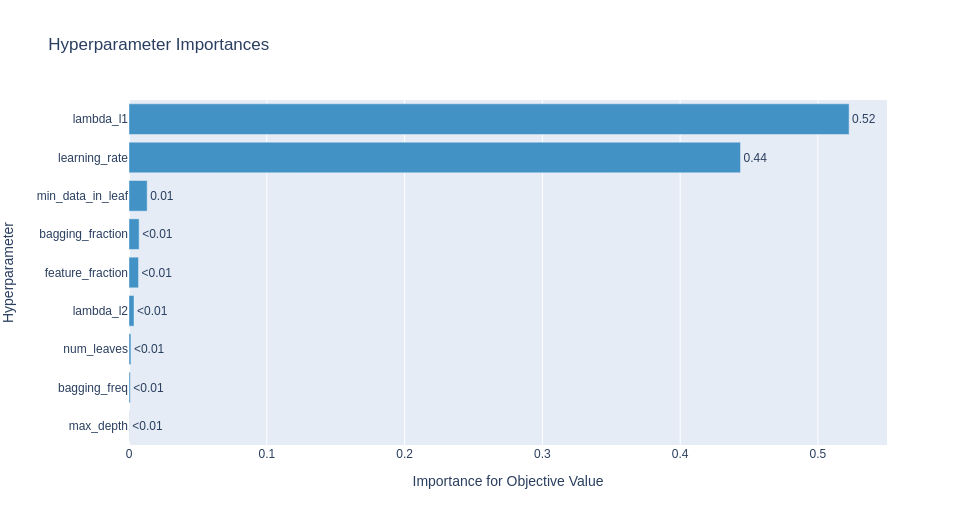
\includegraphics[scale=0.4]{images/importance_lgbm_dia.png}
\end{figure}
Ou seja, podemos concluir que ao longo do estudo do Optuna o hiperparâmetro com maior importância no resultado final foram o \textit{lambda\_l1} e o \textit{learning\_rate}.
% \begin{figure}[H]
%  \caption{Hiperparâmetros \textit{lambda\_l1} do LightGBM no estudo do Optuna no conjunto de dados de Diabetes.}.
%  \label{fig:op:dia:lamb:lgbm}
%  \centering
%  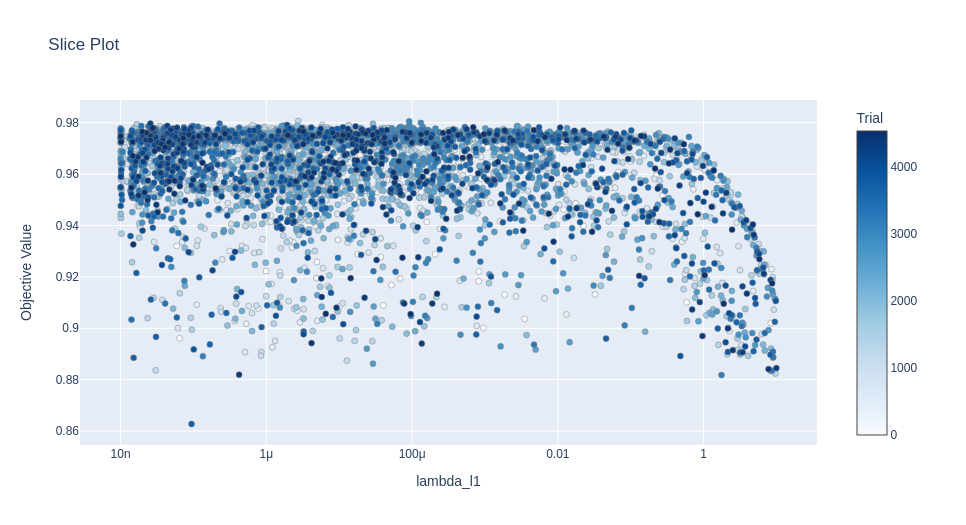
\includegraphics[scale=0.4]{images/optuna_lgbm_lambda_dia.png}
% \end{figure}
% \begin{figure}[H]
%  \caption{Hiperparâmetros \textit{learning\_rate} do LightGBM no estudo do Optuna no conjunto de dados de Diabetes.}.
%  \label{fig:op:dia:learn:lgbm}
%  \centering
%  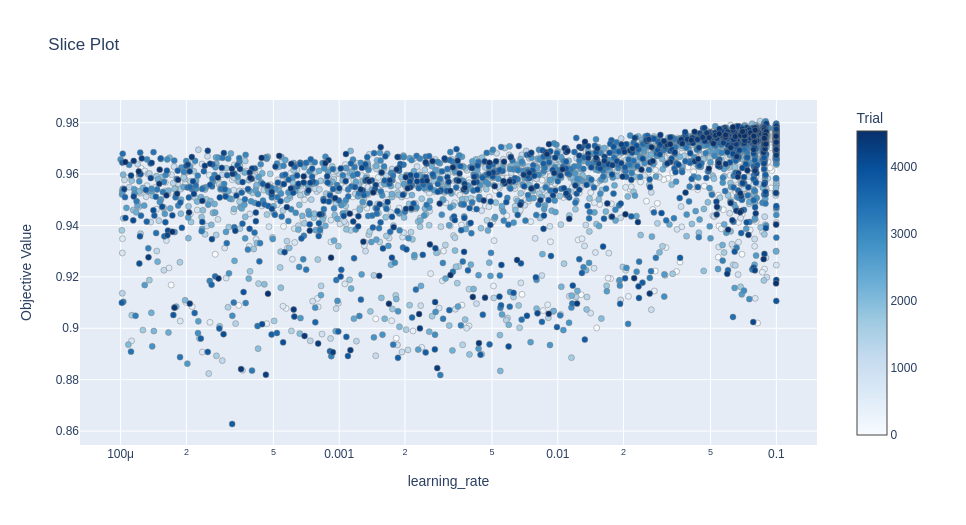
\includegraphics[scale=0.4]{images/optuna_lgbm_learn_dia.png}
% \end{figure}


\section{Resultados Conjunto de dados de Insuficiência Cardíaca}
\begin{table}[H]
\centering
\begin{tabular}{|c|c|c|c|}
\hline
	& \textbf{XGBoost} &\textbf{CatBoost} & \textbf{LightGBM} \\
\hline
\textbf{AUC}	& 0.84930&	0.90048&	0.86291\\
\hline
\textbf{logloss}	& 5.25595&	3.50396	&0.75538\\
\hline
\textbf{KS}	&0.69861	&0.80096	&0.72583\\
\hline
\textbf{tempo (s)}	& 0.13467	&1.41323	&0.06788 \\
\hline
\end{tabular}
\caption{Resultado do XGBoost, CatBoost e LGBM com os hiperparâmetros \textit{Default} no conjunto de dados de insuficiência cardíaca.}\label{res:car:1}
\end{table}

\begin{table}[H]
\label{res:car:2}
\centering
\begin{tabular}{|c|c|c|c|}
\hline
	& \textbf{XGBoost} &\textbf{CatBoost} & \textbf{LightGBM} \\
\hline
\textbf{AUC}	& 0.87021&	0.87631	&0.88219\\
\hline
\textbf{logloss}	& 4.63023&	4.37995&	4.25481\\
\hline
\textbf{KS}	&0.74042	&0.75261&	0.76437\\
\hline
\textbf{tempo (s)}	& 0.10487	&0.92945	&0.05179 \\
\hline
\end{tabular}
\caption{Resultado do XGBoost, CatBoost e LGBM com os hiperparâmetros $LR=0.1$, $MD=3$, $Reg_L=0.01$ no conjunto de dados de insuficiência cardíaca.}
\end{table}

\begin{table}[H]
\label{res:car:3}
\centering
\begin{tabular}{|c|c|c|c|}
\hline
	& \textbf{XGBoost} &\textbf{CatBoost} & \textbf{LightGBM} \\
\hline
\textbf{AUC}	& 0.86738	&0.84745	&0.87021\\
\hline
\textbf{logloss}	& 4.63024&	5.50622	&4.63023\\
\hline
\textbf{KS}	&0.73476	&0.69490	&0.74042\\
\hline
\textbf{tempo (s)}	& 0.12673	&0.90088	&0.10750 \\
\hline
\end{tabular}
\caption{Resultado do XGBoost, CatBoost e LGBM com os hiperparâmetros $LR=0.3$, $MD=3$, $Reg_L=0.01$ no conjunto de dados de insuficiência cardíaca.}
\end{table}

\begin{table}[H]
\label{res:car:4}
\centering
\begin{tabular}{|c|c|c|c|}
\hline
	& \textbf{XGBoost} &\textbf{CatBoost} & \textbf{LightGBM} \\
\hline
\textbf{AUC}	& 0.84016	&0.87348	&0.86574\\
\hline
\textbf{logloss}	& 5.63137&	4.37996	&4.75538\\
\hline
\textbf{KS}	&0.68031	&0.74695	&0.73149\\
\hline
\textbf{tempo (s)}	& 0.09536	&1.42294	&0.06001 \\
\hline
\end{tabular}
\caption{Resultado do XGBoost, CatBoost e LGBM com os hiperparâmetros $LR=0.1$, $MD=6$, $Reg_L=0.01$ no conjunto de dados de insuficiência cardíaca.}
\end{table}

\begin{table}[H]
\label{res:car:5}
\centering
\begin{tabular}{|c|c|c|c|}
\hline
	& \textbf{XGBoost} &\textbf{CatBoost} & \textbf{LightGBM} \\
\hline
\textbf{AUC}	& 0.86879	&0.88850	&0.87043\\
\hline
\textbf{logloss}	& 4.63024	&3.87939	&4.50510\\
\hline
\textbf{KS}	&0.73759&	0.77700&	0.74085\\
\hline
\textbf{tempo (s)}	& 0.11721	&0.94580	&0.08204 \\
\hline
\end{tabular}
\caption{Resultado do XGBoost, CatBoost e LGBM com os hiperparâmetros $LR=0.1$, $MD=3$, $Reg_L=0.05$ no conjunto de dados de insuficiência cardíaca.}
\end{table}

\begin{table}[H]
\label{res:car:6}
\centering
\begin{tabular}{|c|c|c|c|}
\hline
	& \textbf{XGBoost} &\textbf{CatBoost} & \textbf{LightGBM} \\
\hline
\textbf{AUC}	& 0.84016	&0.87348	&0.85965\\
\hline
\textbf{logloss}	& 5.63137	&4.37996	&5.00566\\
\hline
\textbf{KS}	&0.68031&	0.74695	&0.71929\\
\hline
\textbf{tempo (s)}	&0.09273	&1.45088	&0.09684 \\
\hline
\end{tabular}
\caption{Resultado do XGBoost, CatBoost e LGBM com os hiperparâmetros $LR=0.3$, $MD=6$, $Reg_L=0.01$ no conjunto de dados de insuficiência cardíaca.}
\end{table}

\begin{table}[H]
\label{res:car:7}
\centering
\begin{tabular}{|c|c|c|c|}
\hline
	& \textbf{XGBoost} &\textbf{CatBoost} & \textbf{LightGBM} \\
\hline
\textbf{AUC}	& 0.84909&	0.86433	&0.86313\\
\hline
\textbf{logloss}	& 5.38108&	4.75538	&4.63025\\
\hline
\textbf{KS}	&0.69817	&0.72866	&0.72626\\
\hline
\textbf{tempo (s)}	&0.10147	&1.44247	&0.08749 \\
\hline
\end{tabular}
\caption{Resultado do XGBoost, CatBoost e LGBM com os hiperparâmetros $LR=0.3$, $MD=6$, $Reg_L=0.05$ no conjunto de dados de insuficiência cardíaca.}
\end{table}

\begin{table}[H]
\label{res:car:8}
\centering
\begin{tabular}{|c|c|c|c|}
\hline
	& \textbf{XGBoost} &\textbf{CatBoost} & \textbf{LightGBM} \\
\hline
\textbf{AUC}	& 0.85355&	0.85823	&0.88545\\
\hline
\textbf{logloss}	& 5.25594	&5.00566	&4.00453\\
\hline
\textbf{KS}	&0.70710	&0.71646	&0.77091\\
\hline
\textbf{tempo (s)}	&0.09487	&0.87380	&0.07974 \\
\hline
\end{tabular}
\caption{Resultado do XGBoost, CatBoost e LGBM com os hiperparâmetros $LR=0.3$, $MD=3$, $Reg_L=0.05$ no conjunto de dados de insuficiência cardíaca.}
\end{table}

\subsection{Optuna no Conjunto de dados de Insuficiência Cardíaca}
No final da execução o Optuna nos retorna a quantidade de \textit{trials} e qual obteve a melhor performance. Abaixo temos os códigos com as melhores saídas do Optuna de cada modelo.
\begin{codigo}[caption={Resultado do Optuna no conjunto de dados de Insuficiência Cardíaca.}, label={codigo:res:op:dia}, language=Python, breaklines=true]
XGBoost_model = train(X_train, y_train, X_test, y_test, balanced='balanced', method='XGBoost')
Trial 5428 finished with value: 0.9363567073170732 and parameters: {'learning_rate': 0.0027923512828505526, 'max_depth': 11, 'min_child_weight': 6, 'gamma': 1.49842650443622e-06, 'alpha': 3.3380595403852844e-05, 'lambda': 1.4463893324744872, 'colsample_bytree': 0.3115616538843963}. Best is trial 1049 with value: 0.9585204703832753.
...
Trial 1049 finished with value: 0.9555204703832753 and parameters: {'learning_rate': 0.08798533546026498, 'max_depth': 8, 'min_child_weight': 6, 'gamma': 1.0023609559031719e-07, 'alpha': 4.900000133344086e-07, 'lambda': 0.0039762308968834745, 'colsample_bytree': 0.7168230705897498}. Best is trial 1049 with value: 0.9555204703832753.
XGBoost - Optimization using optuna
auc:0.9585204703832753 , log_loss:0.2824692901390929 , ks:0.7900696864111498

CatBoost_model = train(X_train_cat, y_train_cat, X_test_cat, y_test_cat, balanced='balanced', method='CATBoost')
Trial 1071 finished with value: 0.9390243902439025 and parameters: {'learning_rate': 0.0008886403252391745, 'depth': 6, 'max_bin': 369, 'min_data_in_leaf': 90, 'l2_leaf_reg': 7.197661215691214, 'random_strength': 0.05598542767802503, 'bagging_temperature': 6.059262032457767, 'od_type': 'IncToDec', 'od_wait': 32}. Best is trial 645 with value: 0.9501851045296168.
...
Trial 645 finished with value: 0.9501851045296168 and parameters: {'learning_rate': 0.006239961585898258, 'depth': 6, 'max_bin': 376, 'min_data_in_leaf': 90, 'l2_leaf_reg': 9.62802219566606, 'random_strength': 0.4312538078007199, 'bagging_temperature': 2.905228965519412, 'od_type': 'IncToDec', 'od_wait': 50}. Best is trial 645 with value: 0.9501851045296168.
CATBoost - Optimization using optuna
auc:0.9501851045296168 , log_loss:0.30122664951900086 , ks:0.7868031358885018

LGBM_model = train(X_train, y_train, X_test, y_test, balanced='balanced', method='LGBM')
Trial 4574 finished with value: 0.9337979094076655 and parameters: {'learning_rate': 0.0028036602874199667, 'num_leaves': 14, 'lambda_l1': 0.000827098906192435, 'lambda_l2': 5.27506369644634, 'min_data_in_leaf': 24, 'max_depth': 58, 'feature_fraction': 0.5068463692550502, 'bagging_fraction': 0.9295403673354412, 'bagging_freq': 6}. Best is trial 3373 with value: 0.9583514808362369.
...
Trial 3373 finished with value: 0.9583514808362369 and parameters: {'learning_rate': 0.0765705960307223, 'num_leaves': 80, 'lambda_l1': 0.3822971805534857, 'lambda_l2': 3.2542108432719523, 'min_data_in_leaf': 26, 'max_depth': 45, 'feature_fraction': 0.4658823406792122, 'bagging_fraction': 0.9753478288001076, 'bagging_freq': 6}. Best is trial 3373 with value: 0.9583514808362369.
LGBM - Optimization using optuna
auc:0.9583514808362369 , log_loss:0.29086650451368734 , ks:0.8094512195121951
\end{codigo}

\begin{table}[H]
\centering
\begin{tabular}{|c|c|c|c|}
\hline
	& \textbf{XGBoost} &\textbf{CatBoost} & \textbf{LightGBM} \\
\hline
\textbf{AUC}	& 0.95852	&0.95019	&0.95835\\
\hline
\textbf{logloss}	& 0.28247	&0.30123	&0.29087\\
\hline
\textbf{KS}	&0.81598	&0.78680 &0.80945\\
\hline
\end{tabular}
\caption{Resultado do XGBoost, CatBoost e LGBM com os hiperparâmetros otimizados pelo Optuna no conjunto de dados de Insuficiência Cardíaca.}\label{res:car:op}
\end{table}
\subsection{Resultados do estudo do Optuna no conjunto de dados de Insuficiência Cardíaca utilizando o XGBoost.}
Novamente, vamos analisar os resultados do estudo do Optuna.
\begin{figure}[H]
 \caption{Valores do estudo do XGBoost no conjunto de dados de Insuficiência Cardíaca pelo Optuna.}
 \label{fig:op:heart:trials:xgb}
 \centering
 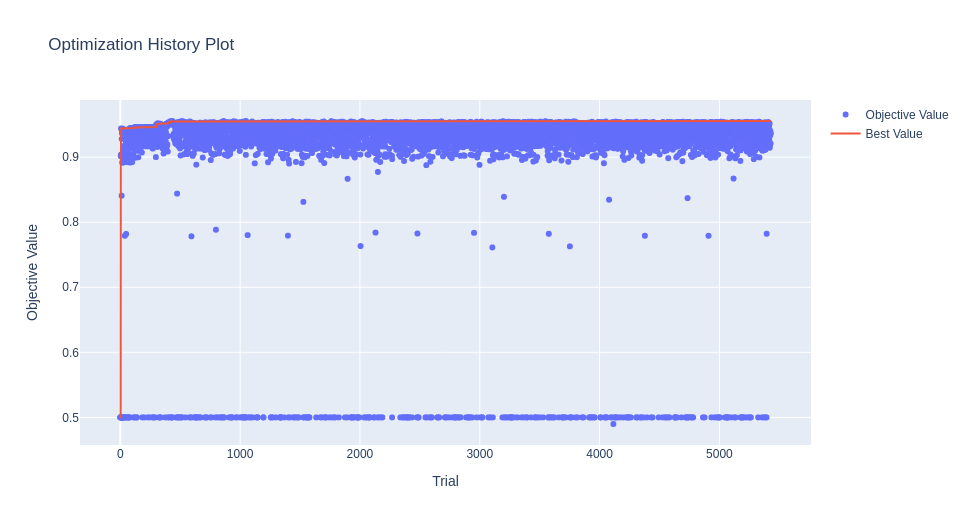
\includegraphics[scale=0.4]{images/optuna_xgboost_heart.png}
\end{figure}
A partir do estudo de otimização do Optuna foi possível identificar quais os hiperparâmetros que possuem o maior impacto no tuning do Optuna.
\begin{figure}[H]
 \caption{Hiperparâmetros do XGBoost com maior importância no Optuna no dados de Insuficiência Cardíaca.}
 \label{fig:op:heart:impo:xgb}
 \centering
 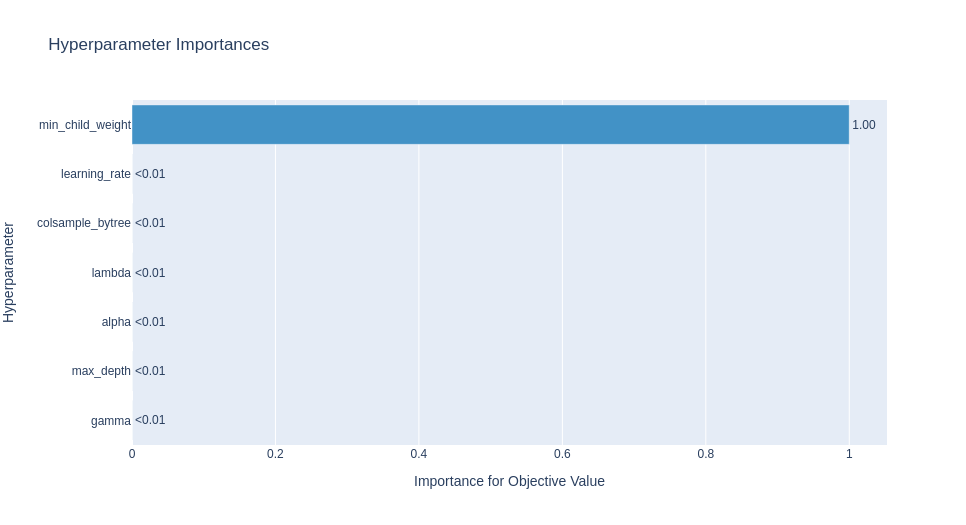
\includegraphics[scale=0.4]{images/optuna_xgboost_importance_heart.png}
\end{figure}
Ou seja, podemos concluir que ao longo do estudo do Optuna o hiperparâmetro com maior importância no resultado final foi o \textit{min\_child\_weight}.
% \begin{figure}[H]
%  \caption{Hiperparâmetros \textit{min\_child\_weight} do XGBoost no estudo do Optuna no conjunto de dados de Insuficiência Cardíaca.}.
%  \label{fig:op:heart:min:xgb}
%  \centering
%  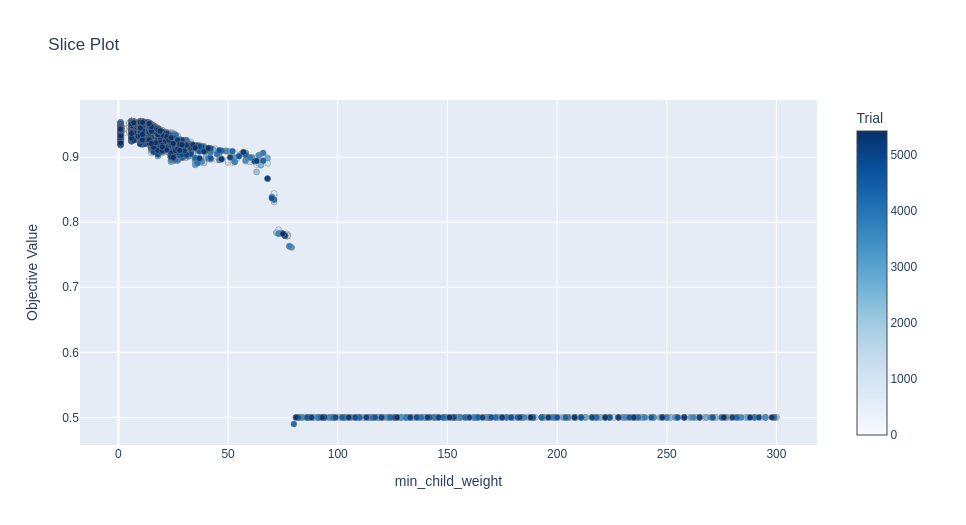
\includegraphics[scale=0.4]{images/optuna_xgboost_min_heart.png}
% \end{figure}

\subsection{Resultados do estudo do Optuna no conjunto de dados de Insuficiência Cardíaca utilizando o CatBoost.}
\begin{figure}[H]
 \caption{Valores do estudo do CatBoost no conjunto de dados de Insuficiência Cardíaca pelo Optuna.}.
 \label{fig:op:heart:trials:cat}
 \centering
 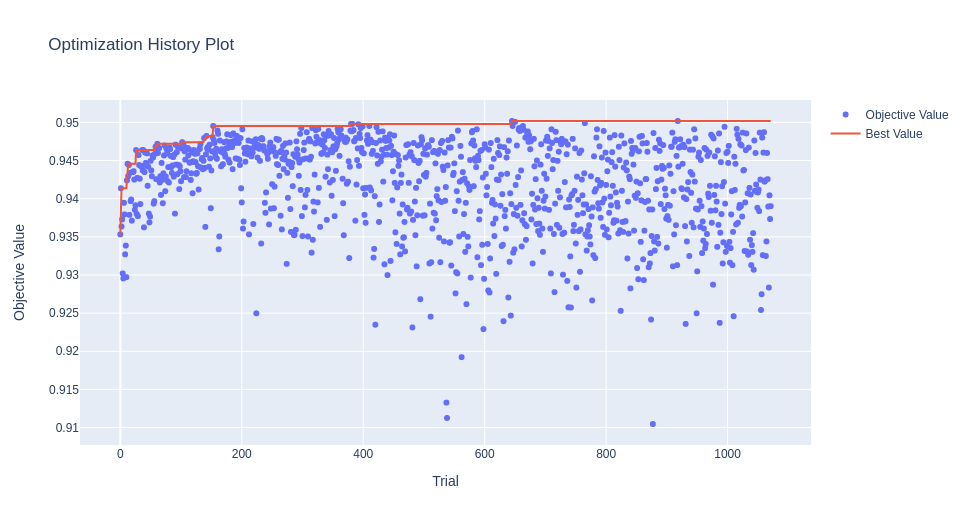
\includegraphics[scale=0.4]{images/optuna_catboost_heart.png}
\end{figure}
A partir do estudo de otimização do Optuna foi possível identificar quais os hiperparâmetros que possuem o maior impacto no tuning do Optuna.
\begin{figure}[H]
 \caption{Hiperparâmetros do XGBoost com maior importância no Optuna no dados de Insuficiência Cardíaca.}
 \label{fig:op:heart:impo:cat}
 \centering
 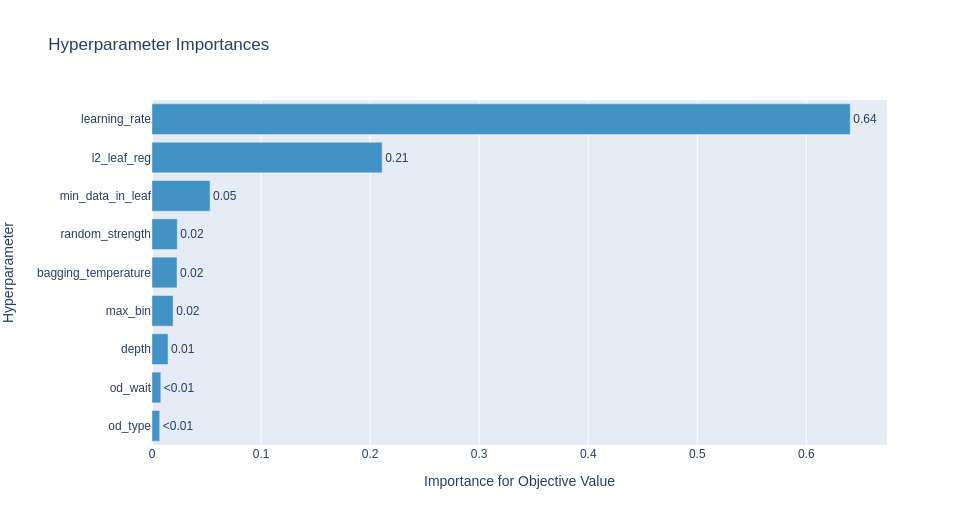
\includegraphics[scale=0.4]{images/optuna_catboost_importance_heart.png}
\end{figure}
Ou seja, podemos concluir que ao longo do estudo do Optuna o hiperparâmetro com maior importância no resultado final foram o \textit{learning\_rate} e o \textit{l2\_leaf\_reg}.
% \begin{figure}[H]
%  \caption{Hiperparâmetros \textit{learning\_rate} do CatBoost no estudo do Optuna no conjunto de dados de Insuficiência Cardíaca.}.
%  \label{fig:op:heart:learn:cat}
%  \centering
%  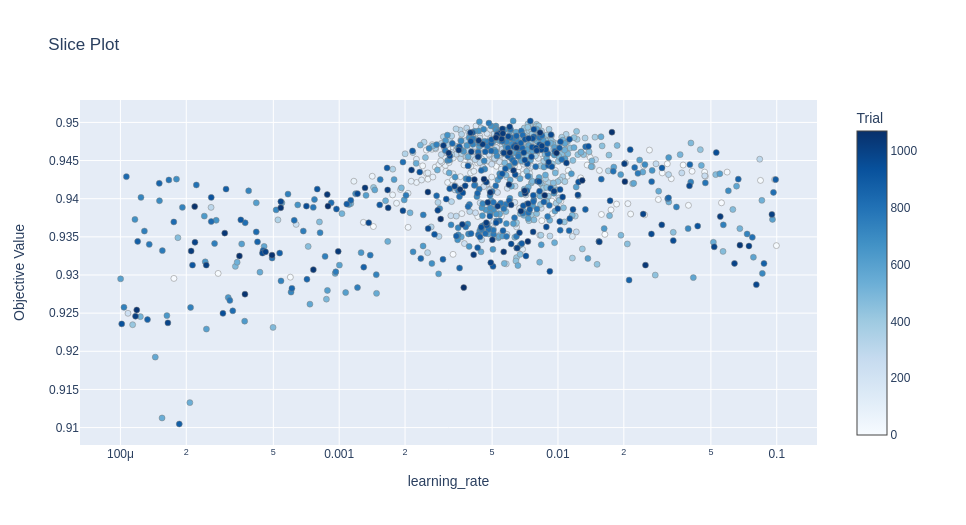
\includegraphics[scale=0.4]{images/optuna_catboost_learning_heart.png}
% \end{figure}
% \begin{figure}[H]
%  \caption{Hiperparâmetros \textit{l2\_leaf\_reg} do CatBoost no estudo do Optuna no conjunto de dados de Insuficiência Cardíaca.}.
%  \label{fig:op:heart:l2:cat}
%  \centering
%  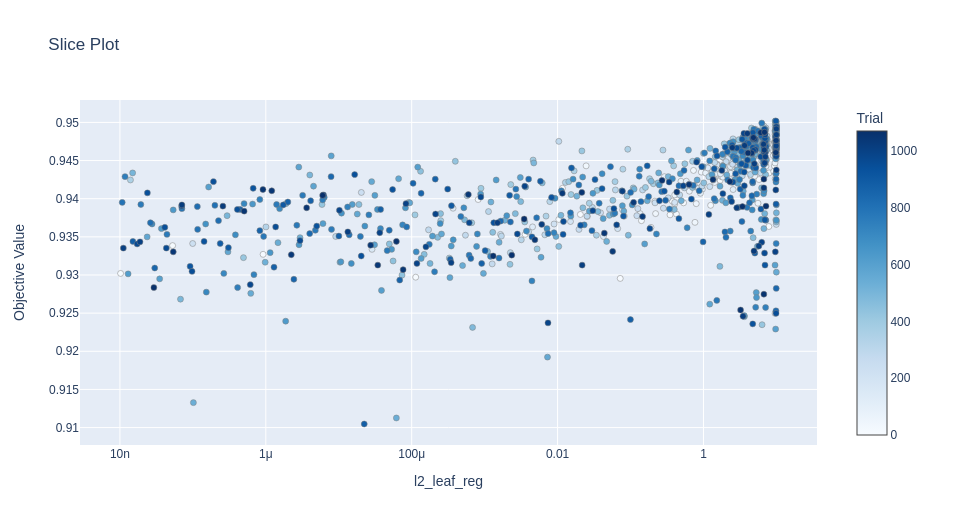
\includegraphics[scale=0.4]{images/optuna_catboost_l2_heart.png}
% \end{figure}

\subsection{Resultados do estudo do Optuna no conjunto de dados de Insuficiência Cardíaca utilizando o LightGBM.}
\begin{figure}[H]
 \caption{Valores do estudo do LightGBM no conjunto de dados de Insuficiência Cardíaca pelo Optuna.}.
 \label{fig:op:heart:trials:lgbm}
 \centering
 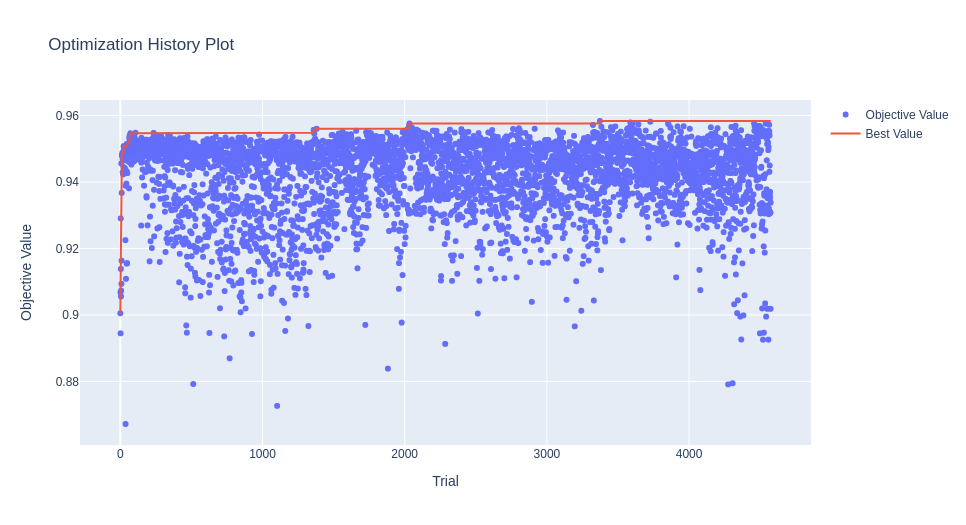
\includegraphics[scale=0.4]{images/optuna_lgbm_heart.png}
\end{figure}
A partir do estudo de otimização do Optuna foi possível identificar quais os hiperparâmetros que possuem o maior impacto no tuning do Optuna.
\begin{figure}[H]
 \caption{Hiperparâmetros do LightGBM com maior importância no Optuna no dados de Insuficiência Cardíaca.}
 \label{fig:op:heart:impo:lgbm}
 \centering
 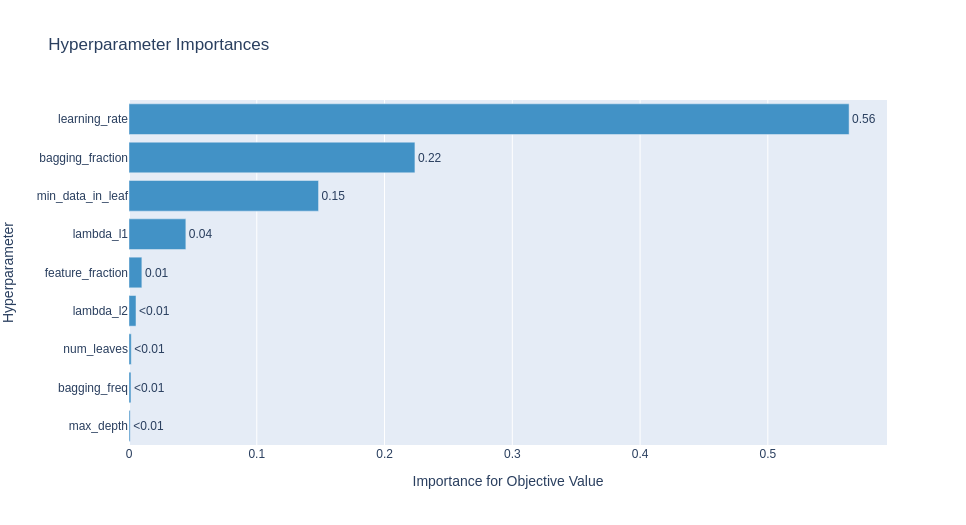
\includegraphics[scale=0.4]{images/optuna_lgbm_importance_heart.png}
\end{figure}
Ou seja, podemos concluir que ao longo do estudo do Optuna o hiperparâmetro com maior importância no resultado final foram o \textit{learning\_rate} e o \textit{min\_data\_in\_leaf}. 
% \begin{figure}[H]
%  \caption{Hiperparâmetros {learning\_rate}  do LightGBM no estudo do Optuna no conjunto de dados de Insuficiência Cardíaca.}.
%  \label{fig:op:heart:learn:lgbm}
%  \centering
%  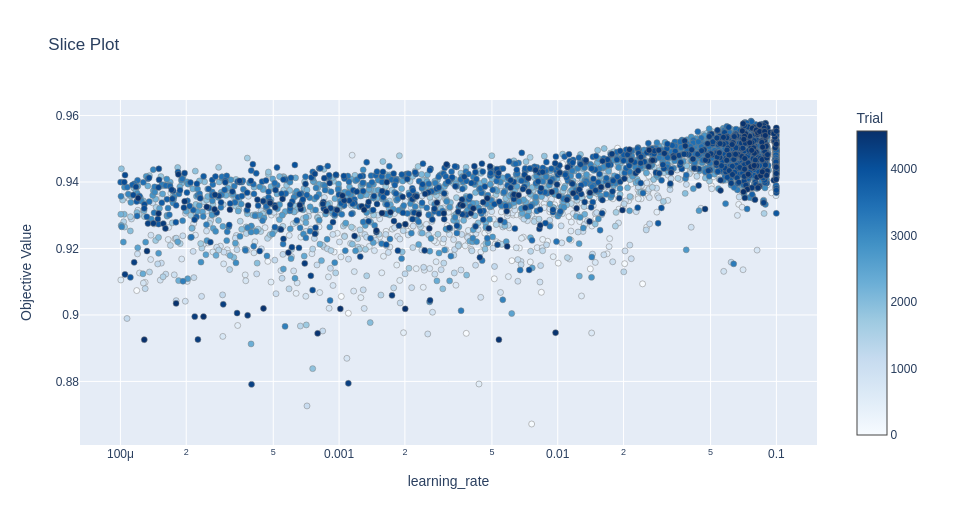
\includegraphics[scale=0.4]{images/optuna_lgbm_learning_heart.png}
% \end{figure}
% \begin{figure}[H]
%  \caption{Hiperparâmetros \textit{min\_data\_in\_leaf} do LightGBM no estudo do Optuna no conjunto de dados de Insuficiência Cardíaca.}.
%  \label{fig:op:heart:min:lgbm}
%  \centering
%  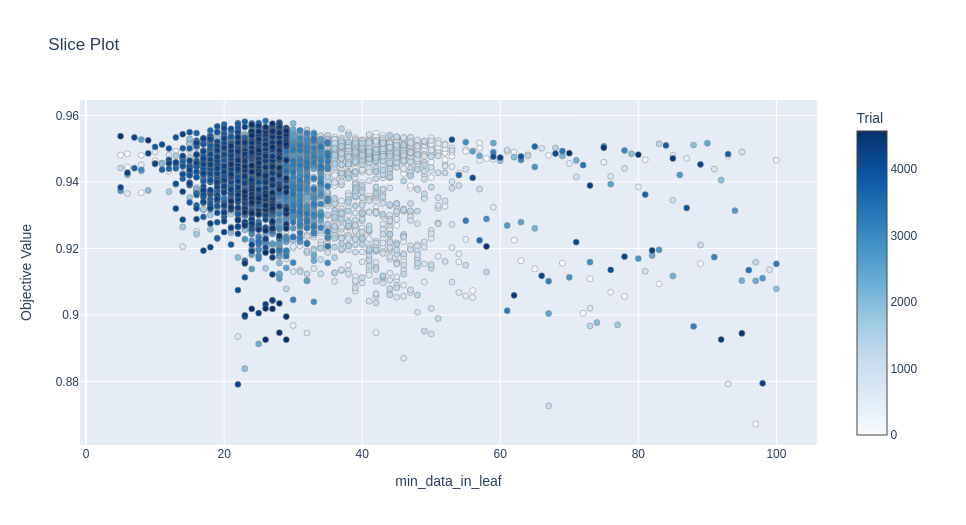
\includegraphics[scale=0.4]{images/optuna_lgbm_min_heart.png}
% \end{figure}

\section{Resultados Conjunto de dados de Insuficiência Renal}
\begin{table}[H]
\centering
\begin{tabular}{|c|c|c|c|}
\hline
	& \textbf{XGBoost} &\textbf{CatBoost} & \textbf{LightGBM} \\
\hline
\textbf{AUC}	& 0.60714&	0.72857	&0.72857\\
\hline
\textbf{logloss}	& 12.95217	&8.63476	&8.63476\\
\hline
\textbf{KS}	&0.21429	&0.45714	&0.45714\\
\hline
\textbf{tempo (s)}	&0.08901	&0.47443	&0.05795 \\
\hline
\end{tabular}
\caption{Resultado do XGBoost, CatBoost e LGBM com os hiperparâmetros \textit{Default} no conjunto de dados de insuficiência renal.}\label{res:ren:1}
\end{table}

\begin{table}[H]
\label{res:ren:2}
\centering
\begin{tabular}{|c|c|c|c|}
\hline
	& \textbf{XGBoost} &\textbf{CatBoost} & \textbf{LightGBM} \\
\hline
\textbf{AUC}	& 0.67857	&0.74286	&0.72857\\
\hline
\textbf{logloss}	& 10.07388	&8.63479	&8.63476\\
\hline
\textbf{KS}	&0.35714&	0.48571&	0.45714\\
\hline
\textbf{tempo (s)}	&0.10748	&0.27430	&0.09398 \\
\hline
\end{tabular}
\caption{Resultado do XGBoost, CatBoost e LGBM com os hiperparâmetros $LR=0.1$, $MD=3$, $Reg_L=0.01$ no conjunto de dados de insuficiência renal.}
\end{table}

\begin{table}[H]
\label{res:ren:3}
\centering
\begin{tabular}{|c|c|c|c|}
\hline
	& \textbf{XGBoost} &\textbf{CatBoost} & \textbf{LightGBM} \\
\hline
\textbf{AUC}	& 0.64286	&0.74286	&0.72857\\
\hline
\textbf{logloss}	& 11.51303	&8.63479	&8.63476\\
\hline
\textbf{KS}	&0.28571	&0.48571	&0.45714\\
\hline
\textbf{tempo (s)}	&0.03914	&0.29207	&0.02660 \\
\hline
\end{tabular}
\caption{Resultado do XGBoost, CatBoost e LGBM com os hiperparâmetros $LR=0.3$, $MD=3$, $Reg_L=0.01$ no conjunto de dados de insuficiência renal.}
\end{table}

\begin{table}[H]
\label{res:ren:4}
\centering
\begin{tabular}{|c|c|c|c|}
\hline
	& \textbf{XGBoost} &\textbf{CatBoost} & \textbf{LightGBM} \\
\hline
\textbf{AUC}	& 0.67857&	0.64286	&0.72857\\
\hline
\textbf{logloss}	& 10.07388	&11.51303	&8.63476\\
\hline
\textbf{KS}	&0.35714	&0.28571	&0.45714\\
\hline
\textbf{tempo (s)}	&0.09602	&0.41013	&0.02825 \\
\hline
\end{tabular}
\caption{Resultado do XGBoost, CatBoost e LGBM com os hiperparâmetros $LR=0.3$, $MD=6$, $Reg_L=0.01$ no conjunto de dados de insuficiência renal.}
\end{table}

\begin{table}[H]
\label{res:ren:5}
\centering
\begin{tabular}{|c|c|c|c|}
\hline
	& \textbf{XGBoost} &\textbf{CatBoost} & \textbf{LightGBM} \\
\hline
\textbf{AUC}	& 0.67857	&0.74286&	0.72857 \\
\hline
\textbf{logloss}	& 10.07388&	8.63479&	8.63476 \\
\hline
\textbf{KS}	&0.35714	&0.48571	&0.45714\\
\hline
\textbf{tempo (s)}	&0.10289	&0.30287	&0.03446 \\
\hline
\end{tabular}
\caption{Resultado do XGBoost, CatBoost e LGBM com os hiperparâmetros $LR=0.1$, $MD=3$, $Reg_L=0.05$ no conjunto de dados de insuficiência renal.}
\end{table}

\begin{table}[H]
\label{res:ren:6}
\centering
\begin{tabular}{|c|c|c|c|}
\hline
	& \textbf{XGBoost} &\textbf{CatBoost} & \textbf{LightGBM} \\
\hline
\textbf{AUC}	& 0.67857&	0.74286&	0.72857 \\
\hline
\textbf{logloss}	& 10.07388	&8.63479&8.63476 \\
\hline
\textbf{KS}	& 0.35714	&0.48571	&0.45714 \\
\hline
\textbf{tempo (s)}	&0.06784&	0.30287	&0.03446 \\
\hline
\end{tabular}
\caption{Resultado do XGBoost, CatBoost e LGBM com os hiperparâmetros $LR=0.3$, $MD=6$, $Reg_L=0.01$ no conjunto de dados de insuficiência renal.}
\end{table}

\begin{table}[H]
\label{res:ren:7}
\centering
\begin{tabular}{|c|c|c|c|}
\hline
	& \textbf{XGBoost} &\textbf{CatBoost} & \textbf{LightGBM} \\
\hline
\textbf{AUC}	& 0.59286&	0.72857	&0.72857 \\
\hline
\textbf{logloss}	& 12.95214	&8.63476&	8.63476 \\
\hline
\textbf{KS}	&0.18571	&0.45714	&0.45714\\
\hline
\textbf{tempo (s)}	&0.05298&	0.40619&	0.07998\\
\hline
\end{tabular}
\caption{Resultado do XGBoost, CatBoost e LGBM com os hiperparâmetros $LR=0.3$, $MD=6$, $Reg_L=0.05$ no conjunto de dados de insuficiência renal.}
\end{table}

\begin{table}[H]
\label{res:ren:8}
\centering
\begin{tabular}{|c|c|c|c|}
\hline
	& \textbf{XGBoost} &\textbf{CatBoost} & \textbf{LightGBM} \\
\hline
\textbf{AUC}	& 0.64286	&0.74286	&0.72857 \\
\hline
\textbf{logloss}	& 11.51303&	8.63479	&8.63476 \\
\hline
\textbf{KS}	&0.28571	&0.48571&	0.45714\\
\hline
\textbf{tempo (s)}	&0.09940&	0.27348	&0.06459 \\
\hline
\end{tabular}
\caption{Resultado do XGBoost, CatBoost e LGBM com os hiperparâmetros $LR=0.3$, $MD=3$, $Reg_L=0.05$ no conjunto de dados de insuficiência renal.}
\end{table}

\subsection{Optuna no Conjunto de dados de Insuficiência Renal}
No final da execução o Optuna nos retorna a quantidade de \textit{trials} e qual obteve a melhor performance. Abaixo temos os códigos com as melhores saídas do Optuna de cada modelo.
\begin{codigo}[caption={Resultado do Optuna no conjunto de dados de Insuficiência Renal.}, label={codigo:res:op:ren}, language=Python, breaklines=true]
XGBoost_model = train(X_train, y_train, X_test, y_test, balanced='balanced', method='XGBoost')
Trial 5455 finished with value: 0.5 and parameters: {'learning_rate': 0.00017538956659154782, 'max_depth': 13, 'min_child_weight': 7, 'gamma': 0.6809045773614, 'alpha': 0.00030549017814601384, 'lambda': 0.0016283305853035024, 'colsample_bytree': 0.7004592509281623}. Best is trial 10 with value: 0.8
...
Trial 10 finished with value: 0.8 and parameters: {'learning_rate': 0.008569334892039517, 'max_depth': 15, 'min_child_weight': 4, 'gamma': 9.423677047435132e-06, 'alpha': 1.185431670644414e-08, 'lambda': 0.012256251224167266, 'colsample_bytree': 0.786661562086467}. Best is trial 10 with value: 0.8.
[I 2023-02-06 18:14:10,324] Trial 11 finished with value: 0.5 and parameters: {'learning_rate': 0.007031543912682467, 'max_depth': 16, 'min_child_weight': 16, 'gamma': 1.0409510458372083e-05, 'alpha': 1.2193044690486938e-08, 'lambda': 0.013018199439117679, 'colsample_bytree': 0.7896246643321345}. Best is trial 10 with value: 0.8.
XGBoost - Optimization using optuna
auc:0.8 , log_loss:0.5702363587915897 , ks:0.5142857142857143

CatBoost_model = train(X_train_cat, y_train_cat, X_test_cat, y_test_cat, balanced='balanced', method='CATBoost')
Trial 2257 finished with value: 0.7785714285714286 and parameters: {'learning_rate': 0.0009648415391471772, 'depth': 6, 'max_bin': 385, 'min_data_in_leaf': 211, 'l2_leaf_reg': 1.6926351852497825, 'random_strength': 3.143996435524371, 'bagging_temperature': 4.896899901794452, 'od_type': 'IncToDec', 'od_wait': 48}. Best is trial 147 with value: 0.9.
...
Trial 147 finished with value: 0.9 and parameters: {'learning_rate': 0.07537894328903638, 'depth': 5, 'max_bin': 358, 'min_data_in_leaf': 248, 'l2_leaf_reg': 1.2327052318936288e-07, 'random_strength': 0.49381984936103734, 'bagging_temperature': 7.0491042648346, 'od_type': 'IncToDec', 'od_wait': 43}. Best is trial 147 with value: 0.9.
CATBoost - Optimization using optuna
auc:0.9 , log_loss:0.9651209210448068 , ks:0.7142857142857143

LGBM_model = train(X_train, y_train, X_test, y_test, balanced='balanced', method='LGBM')
Trial 4753 finished with value: 0.8214285714285714 and parameters: {'learning_rate': 0.04666777939260228, 'num_leaves': 150, 'lambda_l1': 2.0584202047356643e-06, 'lambda_l2': 2.6949988611136263e-08, 'min_data_in_leaf': 7, 'max_depth': 62, 'feature_fraction': 0.7016619725081281, 'bagging_fraction': 0.6273888361729247, 'bagging_freq': 7}. Best is trial 426 with value: 0.8857142857142858.
...
Trial 426 finished with value: 0.8857142857142858 and parameters: {'learning_rate': 0.08959873811059711, 'num_leaves': 186, 'lambda_l1': 3.78113915153367e-08, 'lambda_l2': 5.286213387951746e-08, 'min_data_in_leaf': 11, 'max_depth': 23, 'feature_fraction': 0.5167806798611404, 'bagging_fraction': 0.6306577516857322, 'bagging_freq': 7}. Best is trial 426 with value: 0.8857142857142858.
LGBM - Optimization using optuna
auc:0.8857142857142858 , log_loss:0.43692623324540775 , ks:0.7285714285714286
\end{codigo}

\begin{table}[H]
\centering
\begin{tabular}{|c|c|c|c|}
\hline
	& \textbf{XGBoost} &\textbf{CatBoost} & \textbf{LightGBM} \\
\hline
\textbf{AUC}	& 0.80000	&0.90000&	0.88571 \\
\hline
\textbf{logloss}	& 0.57024	& 0.96512 &	0.43693\\
\hline
\textbf{KS}	&0.51429&	0.71429	& 0.72857\\
\hline
\end{tabular}
\caption{Resultado do XGBoost, CatBoost e LGBM com os hiperparâmetros otimizados pelo Optuna no conjunto de dados de Insuficiência Renal.}\label{res:ren:op}
\end{table}
\subsection{Resultados do estudo do Optuna no conjunto de dados de Insuficiência Renal utilizando o XGBoost.}
Novamente, vamos analisar os resultados do estudo do Optuna.
\begin{figure}[H]
 \caption{Valores do estudo do XGBoost no conjunto de dados de Insuficiência Renal pelo Optuna.}
 \label{fig:op:kind:trials:xgb}
 \centering
 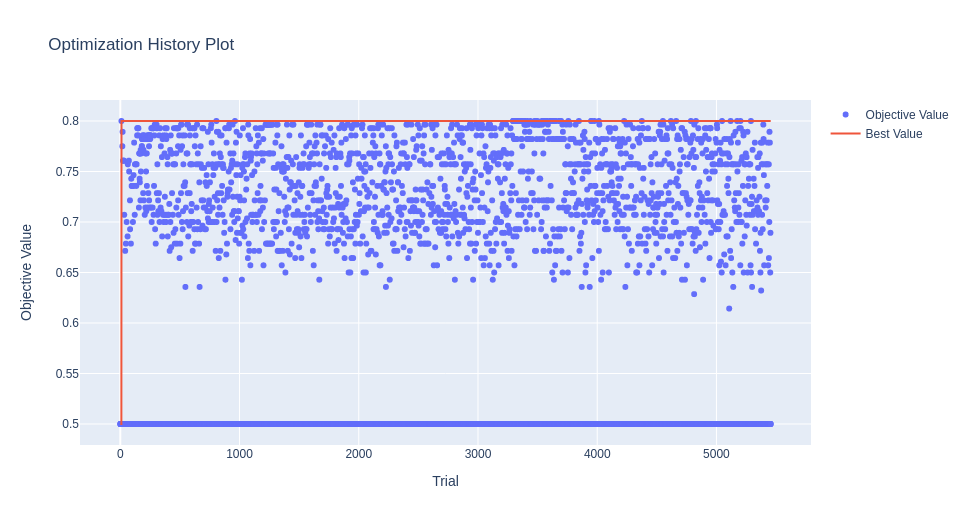
\includegraphics[scale=0.4]{images/optuna_xgboost_kindey.png}
\end{figure}
A partir do estudo de otimização do Optuna foi possível identificar quais os hiperparâmetros que possuem o maior impacto no tuning do Optuna.
\begin{figure}[H]
 \caption{Hiperparâmetros do XGBoost com maior importância no Optuna no dados de Insuficiência Renal.}
 \label{fig:op:kind:impo:xgb}
 \centering
 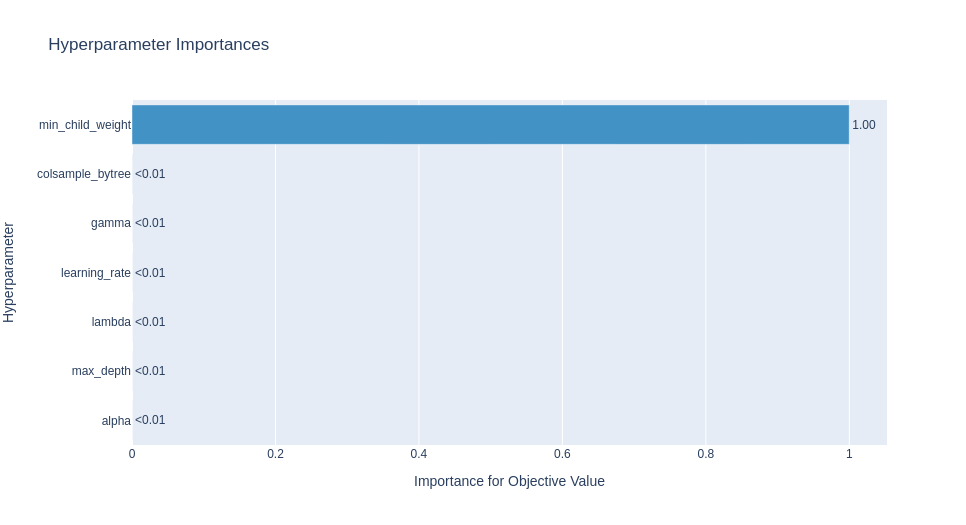
\includegraphics[scale=0.4]{images/optuna_xgboost_importance_kidney.png}
\end{figure}
Ou seja, podemos concluir que ao longo do estudo do Optuna o hiperparâmetro com maior importância no resultado final foi o \textit{min\_child\_weight}.
% \begin{figure}[H]
%  \caption{Hiperparâmetros \textit{min\_child\_weight} do XGBoost no estudo do Optuna no conjunto de dados de Insuficiência Renal.}.
%  \label{fig:op:kind:min:xgb}
%  \centering
%  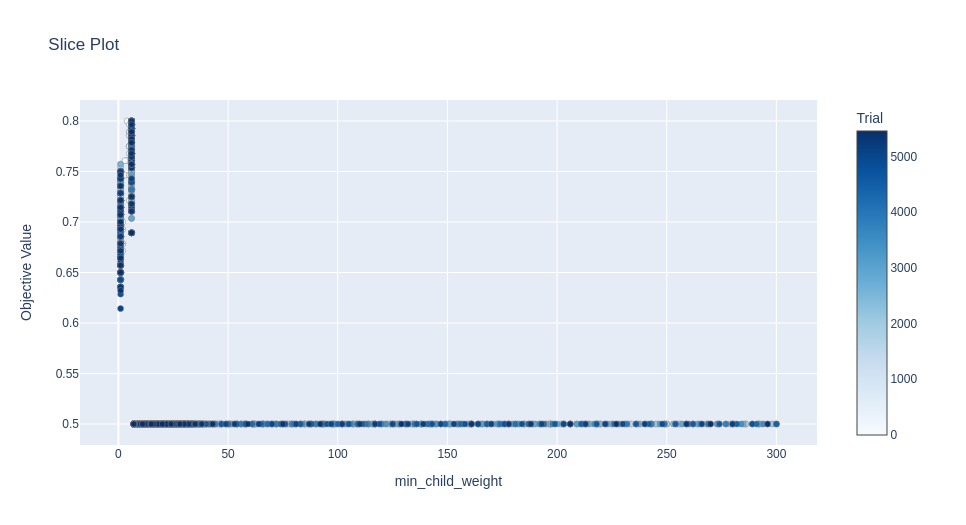
\includegraphics[scale=0.4]{images/optuna_min_xgboost_kindey.png}
% \end{figure}

\subsection{Resultados do estudo do Optuna no conjunto de dados de Insuficiência Renal utilizando o CatBoost.}
\begin{figure}[H]
 \caption{Valores do estudo do CatBoost no conjunto de dados de Insuficiência Renal pelo Optuna.}
 \label{fig:op:kind:trials:cat}
 \centering
 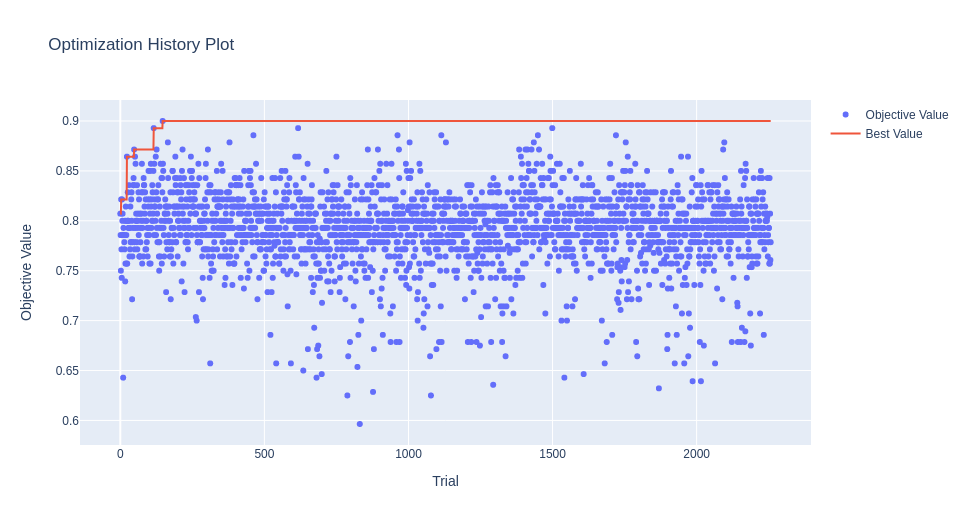
\includegraphics[scale=0.4]{images/optuna_catboost_kidney.png}
\end{figure}
A partir do estudo de otimização do Optuna foi possível identificar quais os hiperparâmetros que possuem o maior impacto no tuning do Optuna.
\begin{figure}[H]
 \caption{Hiperparâmetros do XGBoost com maior importância no Optuna no dados de Insuficiência Renal.}
 \label{fig:op:kind:impo:cat}
 \centering
 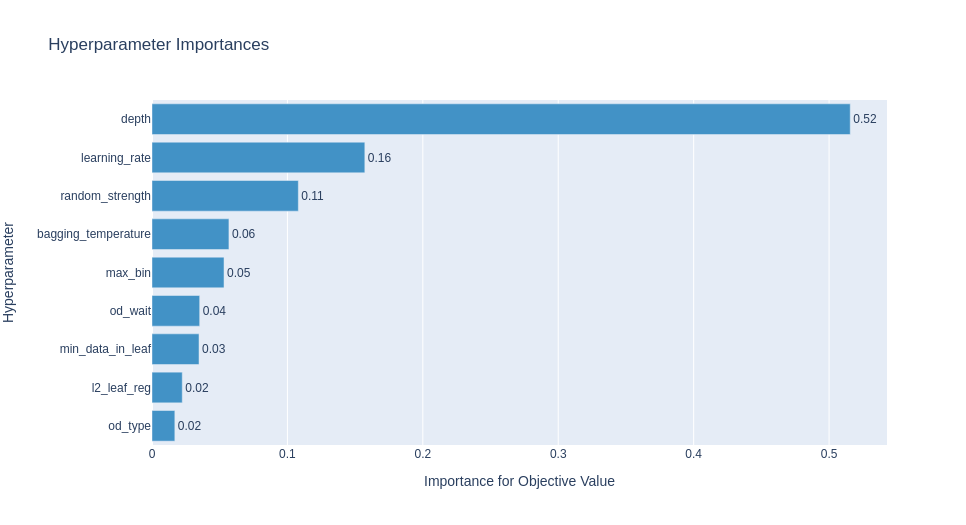
\includegraphics[scale=0.4]{images/optuna_catboost_importance_kidney.png}
\end{figure}
Ou seja, podemos concluir que ao longo do estudo do Optuna o hiperparâmetro com maior importância no resultado final foram o \textit{depth} e o \textit{learning\_rate}.
% \begin{figure}[H]
%  \caption{Hiperparâmetros \textit{depth} do CatBoost no estudo do Optuna no conjunto de dados de Insuficiência Renal.}.
%  \label{fig:op:kind:depth:cat}
%  \centering
%  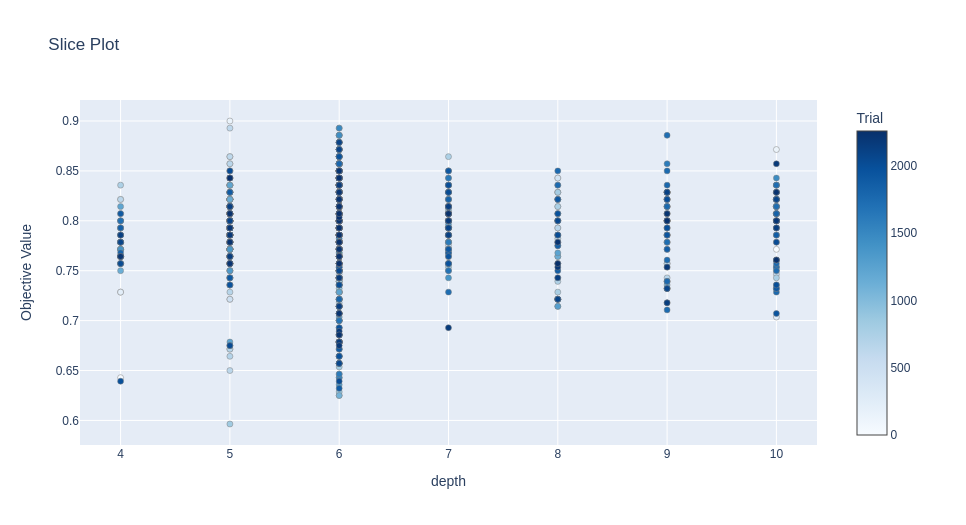
\includegraphics[scale=0.4]{images/opatuna_catboost_depth_kindey.png}
% \end{figure}
% \begin{figure}[H]
%  \caption{Hiperparâmetros \textit{learning\_rate} do CatBoost no estudo do Optuna no conjunto de dados de Insuficiência Renal.}.
%  \label{fig:op:kind:learn:cat}
%  \centering
%  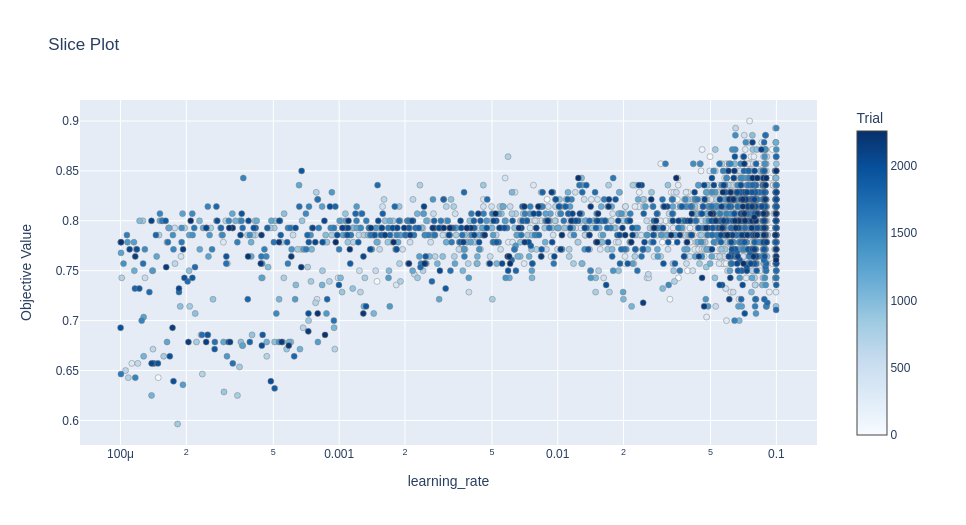
\includegraphics[scale=0.4]{images/optuna_learning_rate-catboost_kindey.png}
% \end{figure}

\subsection{Resultados do estudo do Optuna no conjunto de dados de Insuficiência Renal utilizando o LightGBM.}
\begin{figure}[H]
 \caption{Valores do estudo do LightGBM no conjunto de dados de Insuficiência Renal pelo Optuna.}
 \label{fig:op:kind:trials:lgbm}
 \centering
 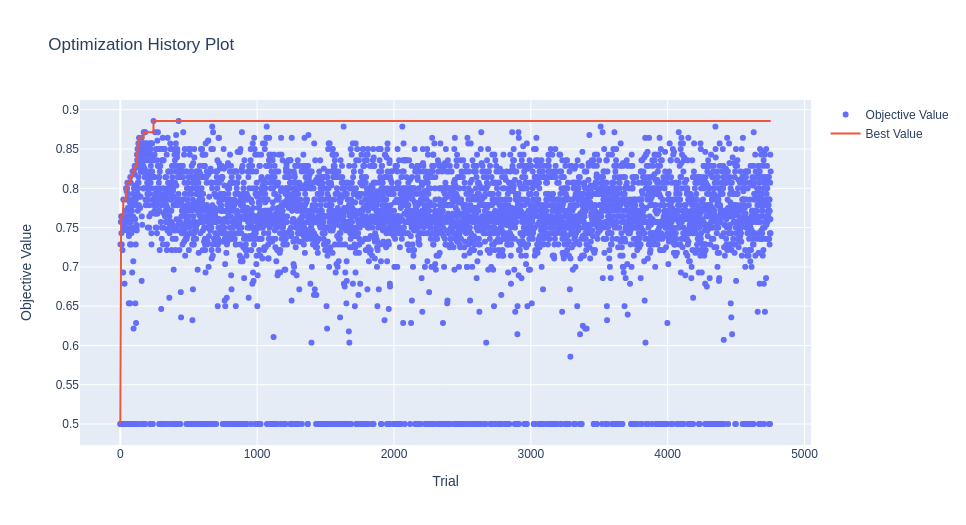
\includegraphics[scale=0.4]{images/optuna_lgbm_kikndey.png}
\end{figure}
A partir do estudo de otimização do Optuna foi possível identificar quais os hiperparâmetros que possuem o maior impacto no tuning do Optuna.
\begin{figure}[H]
 \caption{Hiperparâmetros do LightGBM com maior importância no Optuna no dados de Insuficiência Renal.}
 \label{fig:op:kind:impo:lgbm}
 \centering
 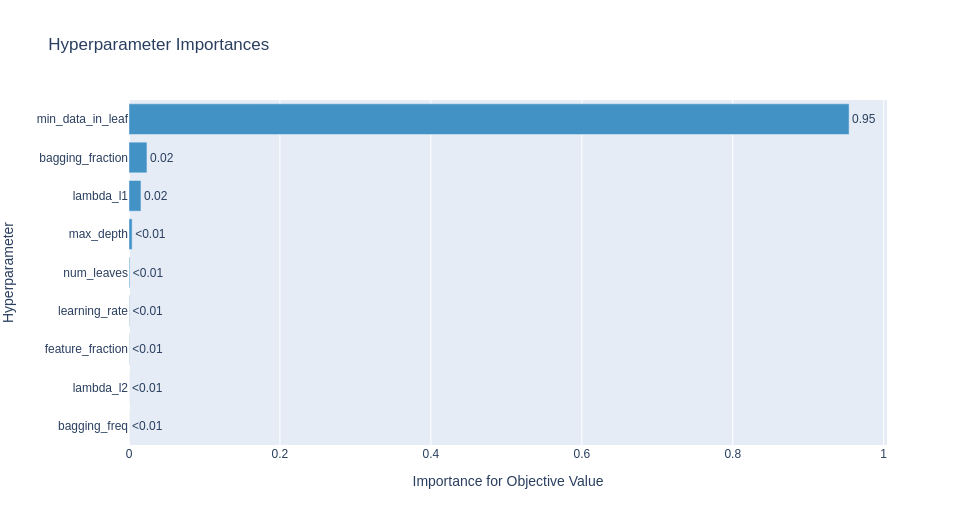
\includegraphics[scale=0.4]{images/optuna_lgbm_importance_kindey.png}
\end{figure}
Ou seja, podemos concluir que ao longo do estudo do Optuna o hiperparâmetro com maior importância no resultado final foi o \textit{min\_data\_in\_leaf}.
% \begin{figure}[H]
%  \caption{Hiperparâmetros \textit{min\_data\_in\_leaf} do LightGBM no estudo do Optuna no conjunto de dados de Insuficiência Renal.}.
%  \label{fig:op:kind:min:lgbm}
%  \centering
%  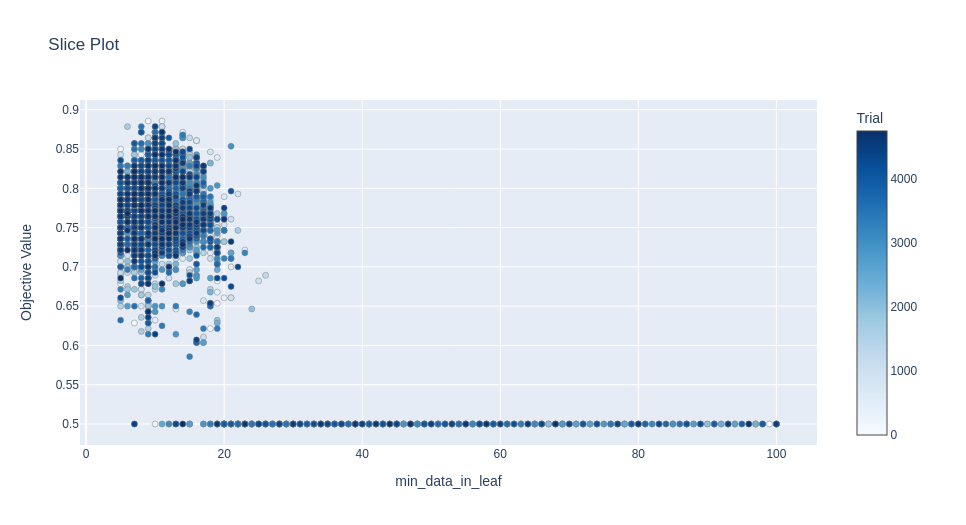
\includegraphics[scale=0.4]{images/optuna_min_lgbm_kindey.png}
% \end{figure}

\section{Resultados Conjunto de dados de Carcinoma de Mama}
\begin{table}[H]
\centering
\begin{tabular}{|c|c|c|c|}
\hline
	& \textbf{XGBoost} &\textbf{CatBoost} & \textbf{LightGBM} \\
\hline
\textbf{AUC}	& 0.97950	&0.97156	&0.94511 \\
\hline
\textbf{logloss}	&0.60595	&0.80793&	1.81785 \\
\hline
\textbf{KS}	&0.95899	&0.94312	&0.89021 \\
\hline
\textbf{tempo (s)}	&0.14904	&2.72823	&0.08682 \\
\hline
\end{tabular}
\caption{Resultado do XGBoost, CatBoost e LGBM com os hiperparâmetros \textit{Default} no conjunto de dados de Carcinoma de Mama.}\label{res:can:1}
\end{table}

\begin{table}[H]
\label{res:ren:2}
\centering
\begin{tabular}{|c|c|c|c|}
\hline
	& \textbf{XGBoost} &\textbf{CatBoost} & \textbf{LightGBM} \\
\hline
\textbf{AUC}	& 0.96693&	0.95899 &	0.95106 \\
\hline
\textbf{logloss}	& 1.00992&	1.21190&	1.41388 \\
\hline
\textbf{KS}	&0.93386&	0.91799	&0.90212 \\
\hline
\textbf{tempo (s)}	&0.08013	&0.81609	&0.10254 \\
\hline
\end{tabular}
\caption{Resultado do XGBoost, CatBoost e LGBM com os hiperparâmetros $LR=0.1$, $MD=3$, $Reg_L=0.01$ no conjunto de dados de Carcinoma de Mama.}
\end{table}

\begin{table}[H]
\label{res:ren:2}
\centering
\begin{tabular}{|c|c|c|c|}
\hline
	& \textbf{XGBoost} &\textbf{CatBoost} & \textbf{LightGBM} \\
\hline
\textbf{AUC}	& 0.96693&	0.95899 &	0.95106 \\
\hline
\textbf{logloss}	& 1.00992&	1.21190&	1.41388 \\
\hline
\textbf{KS}	&0.93386&	0.91799	&0.90212 \\
\hline
\textbf{tempo (s)}	&0.08013	&0.81609	&0.10254 \\
\hline
\end{tabular}
\caption{Resultado do XGBoost, CatBoost e LGBM com os hiperparâmetros $LR=0.1$, $MD=3$, $Reg_L=0.01$ no conjunto de dados de Carcinoma de Mama.}
\end{table}

\begin{table}[H]
\label{res:ren:3}
\centering
\begin{tabular}{|c|c|c|c|}
\hline
	& \textbf{XGBoost} &\textbf{CatBoost} & \textbf{LightGBM} \\
\hline
\textbf{AUC}	& 0.97487	&0.95437	&0.95106 \\
\hline
\textbf{logloss}	& 0.80793	&1.41388	&1.41388 \\
\hline
\textbf{KS}	& 0.94974	&0.90873	&0.90212 \\
\hline
\textbf{tempo (s)}	& 0.10812	&0.78369	&0.07552 \\
\hline
\end{tabular}
\caption{Resultado do XGBoost, CatBoost e LGBM com os hiperparâmetros $LR=0.3$, $MD=3$, $Reg_L=0.01$ no conjunto de dados de Carcinoma de Mama.}
\end{table}

\begin{table}[H]
\label{res:ren:4}
\centering
\begin{tabular}{|c|c|c|c|}
\hline
	& \textbf{XGBoost} &\textbf{CatBoost} & \textbf{LightGBM} \\
\hline
\textbf{AUC}	& 0.96362&	0.97156	&0.95899 \\
\hline
\textbf{logloss}	& 1.00991	&0.80793	&1.21190 \\
\hline
\textbf{KS}	&0.92725	&0.94312	&0.91799 \\
\hline
\textbf{tempo (s)}	&0.09410	&3.08160	&0.05303\\
\hline
\end{tabular}
\caption{Resultado do XGBoost, CatBoost e LGBM com os hiperparâmetros $LR=0.1$, $MD=6$, $Reg_L=0.01$ no conjunto de dados de Carcinoma de Mama.}
\end{table}

\begin{table}[H]
\label{res:ren:5}
\centering
\begin{tabular}{|c|c|c|c|}
\hline
	& \textbf{XGBoost} &\textbf{CatBoost} & \textbf{LightGBM} \\
\hline
\textbf{AUC}	&0.95899	&0.96362	&0.95106 \\
\hline
\textbf{logloss}	& 1.21190	&1.00991	&1.41388\\
\hline
\textbf{KS}	&0.91799	&0.92725	&0.90212 \\
\hline
\textbf{tempo (s)}	&0.09263	&0.77307&	0.08819 \\
\hline
\end{tabular}
\caption{Resultado do XGBoost, CatBoost e LGBM com os hiperparâmetros $LR=0.1$, $MD=3$, $Reg_L=0.05$ no conjunto de dados de Carcinoma de Mama.}
\end{table}

\begin{table}[H]
\label{res:ren:6}
\centering
\begin{tabular}{|c|c|c|c|}
\hline
	& \textbf{XGBoost} &\textbf{CatBoost} & \textbf{LightGBM} \\
\hline
\textbf{AUC}	& 0.97156	&0.95899	&0.95437 \\
\hline
\textbf{logloss}	& 0.80793	&1.21190	&1.41388 \\
\hline
\textbf{KS}	&0.94312	&0.91799	&0.90873 \\
\hline
\textbf{tempo (s)}	&0.08900	&2.68093	&0.07608\\
\hline
\end{tabular}
\caption{Resultado do XGBoost, CatBoost e LGBM com os hiperparâmetros $LR=0.3$, $MD=6$, $Reg_L=0.01$ no conjunto de dados de Carcinoma de Mama.}
\end{table}

\begin{table}[H]
\label{res:ren:7}
\centering
\begin{tabular}{|c|c|c|c|}
\hline
	& \textbf{XGBoost} &\textbf{CatBoost} & \textbf{LightGBM} \\
\hline
\textbf{AUC}	& 0.97156&	0.97156	&0.06191 \\
\hline
\textbf{logloss}	& 0.80793	&0.80793&	0.95899 \\
\hline
\textbf{KS}	&0.94312	&0.94312&	1.21190\\
\hline
\textbf{tempo (s)}	&0.07007&	2.72953	&0.91799\\
\hline
\end{tabular}
\caption{Resultado do XGBoost, CatBoost e LGBM com os hiperparâmetros $LR=0.3$, $MD=6$, $Reg_L=0.05$ no conjunto de dados de Carcinoma de Mama.}
\end{table}

\begin{table}[H]
\label{res:ren:8}
\centering
\begin{tabular}{|c|c|c|c|}
\hline
	& \textbf{XGBoost} &\textbf{CatBoost} & \textbf{LightGBM} \\
\hline
\textbf{AUC}	& 0.96693	&0.95437	&0.95106 \\
\hline
\textbf{logloss}	& 1.00992&	1.41388	&1.41388 \\
\hline
\textbf{KS}	&0.93386	&0.90873	&0.90212 \\
\hline
\textbf{tempo (s)}	&0.05206&	0.83468	&0.09816\\
\hline
\end{tabular}
\caption{Resultado do XGBoost, CatBoost e LGBM com os hiperparâmetros $LR=0.3$, $MD=3$, $Reg_L=0.05$ no conjunto de dados de Carcinoma de Mama.}
\end{table}


\subsection{Optuna no Conjunto de dados de Carcinoma de Mama}
No final da execução o Optuna nos retorna a quantidade de \textit{trials} e qual obteve a melhor performance. Abaixo temos os códigos com as melhores saídas do Optuna de cada modelo.
\begin{codigo}[caption={Resultado do Optuna no conjunto de dados de Carcinoma de Mama.}, label={codigo:res:op:can}, language=Python, breaklines=true]
XGBoost_model = train(X_train, y_train, X_test, y_test, balanced='balanced', method='XGBoost')
Trial 4948 finished with value: 0.9972075249853027 and parameters: {'learning_rate': 0.05731935932209517, 'max_depth': 11, 'min_child_weight': 6, 'gamma': 3.4052496218231224e-05, 'alpha': 3.790159562548499e-08, 'lambda': 0.37064484949542936, 'colsample_bytree': 0.1368272730789507}. Best is trial 615 with value: 0.9988242210464433.
...
Trial 615 finished with value: 0.9988242210464433 and parameters: {'learning_rate': 0.0436689491255323, 'max_depth': 14, 'min_child_weight': 15, 'gamma': 3.027611637978531e-07, 'alpha': 1.2966964481647062e-07, 'lambda': 1.125613997027746, 'colsample_bytree': 0.13844700517507155}. Best is trial 615 with value: 0.9988242210464433.
XGBoost - Optimization using optuna
auc:0.9988242210464433 , log_loss:0.1163896211145217 , ks:0.9841269841269841

CatBoost_model = train(X_train_cat, y_train_cat, X_test_cat, y_test_cat, balanced='balanced', method='CATBoost')
Trial 350 finished with value: 0.9975014697236919 and parameters: {'learning_rate': 0.014693012954604871, 'depth': 6, 'max_bin': 371, 'min_data_in_leaf': 128, 'l2_leaf_reg': 1.6337878324887535e-05, 'random_strength': 5.267279748486068, 'bagging_temperature': 8.30501182209448, 'od_type': 'Iter', 'od_wait': 31}. Best is trial 71 with value: 0.9992651381540271.
...
Trial 71 finished with value: 0.9992651381540271 and parameters: {'learning_rate': 0.006920317042180218, 'depth': 6, 'max_bin': 375, 'min_data_in_leaf': 18, 'l2_leaf_reg': 5.356718213907343e-06, 'random_strength': 7.0698333503761, 'bagging_temperature': 8.330048758136687, 'od_type': 'Iter', 'od_wait': 30}. Best is trial 71 with value: 0.9992651381540271.
CATBoost - Optimization using optuna
auc:0.9992651381540271 , log_loss:0.044536185929194914 , ks:0.9748677248677248

LGBM_model = train(X_train, y_train, X_test, y_test, balanced='balanced', method='LGBM')
Trial 4658 finished with value: 0.9961787184009405 and parameters: {'learning_rate': 0.0739594630318519, 'num_leaves': 142, 'lambda_l1': 6.1038128339002564e-06, 'lambda_l2': 1.0045566613521662e-08, 'min_data_in_leaf': 61, 'max_depth': 9, 'feature_fraction': 0.41696597857129664, 'bagging_fraction': 0.8138570308199493, 'bagging_freq': 4}. Best is trial 2418 with value: 0.9994121105232218.
...
Trial 2418 finished with value: 0.9994121105232218 and parameters: {'learning_rate': 0.07615521372640538, 'num_leaves': 219, 'lambda_l1': 2.74036247131309e-08, 'lambda_l2': 1.7948089596435946e-07, 'min_data_in_leaf': 66, 'max_depth': 18, 'feature_fraction': 0.4971540914007164, 'bagging_fraction': 0.43488273051341403, 'bagging_freq': 4}. Best is trial 2418 with value: 0.9994121105232218.
LGBM - Optimization using optuna
auc:0.9994121105232218 , log_loss:0.06707615388690602 , ks:0.9841269841269841
\end{codigo}

\begin{table}[H]
\centering
\begin{tabular}{|c|c|c|c|}
\hline
	& \textbf{XGBoost} &\textbf{CatBoost} & \textbf{LightGBM} \\
\hline
\textbf{AUC}	& 0.99882 &	0.99927 &0.99941 \\
\hline
\textbf{logloss}	& 0.11639	&0.04454 &	0.06708 \\
\hline
\textbf{KS}	&0.98413	&0.97487 &	0.98413 \\
\hline
\end{tabular}
\caption{Resultado do XGBoost, CatBoost e LGBM com os hiperparâmetros otimizados pelo Optuna no conjunto de dados de Carcinoma de Mama.}\label{res:can:op}
\end{table}

\subsection{Resultados do estudo do Optuna no conjunto de dados de Carcinoma de Mama utilizando o XGBoost.}
Novamente iremos analisar o estudo do Optuna.
\begin{figure}[H]
 \caption{Valores do estudo do XGBoost no conjunto de dados de Carcinoma de Mama pelo Optuna.}.
 \label{fig:op:cancer:trials:xgb}
 \centering
 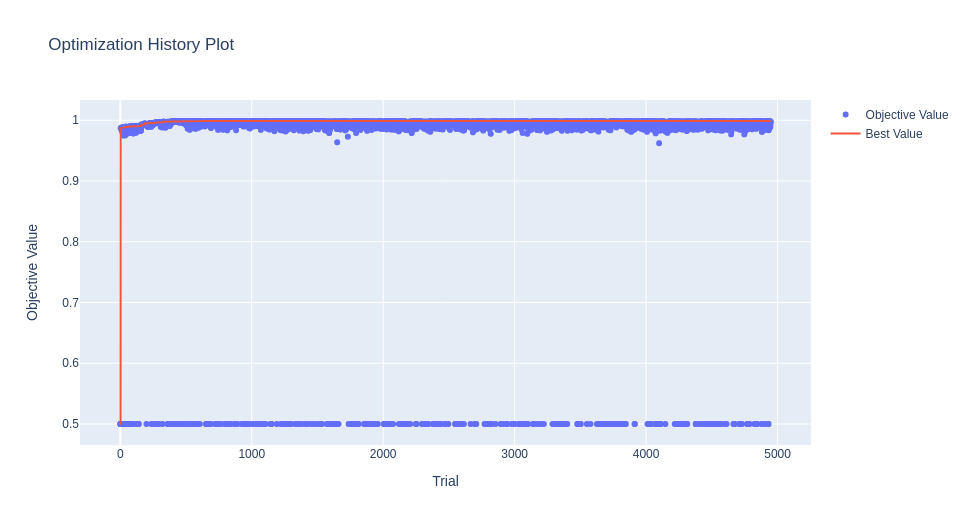
\includegraphics[scale=0.4]{images/optuna_xgboost_cancer.png}
\end{figure}
A partir do estudo de otimização do Optuna foi possível identificar quais os hiperparâmetros que possuem o maior impacto no tuning do Optuna.
\begin{figure}[H]
 \caption{Hiperparâmetros do XGBoost com maior importância no Optuna no dados de Carcinoma de Mama.}
 \label{fig:op:cancer:impo:xgb}
 \centering
 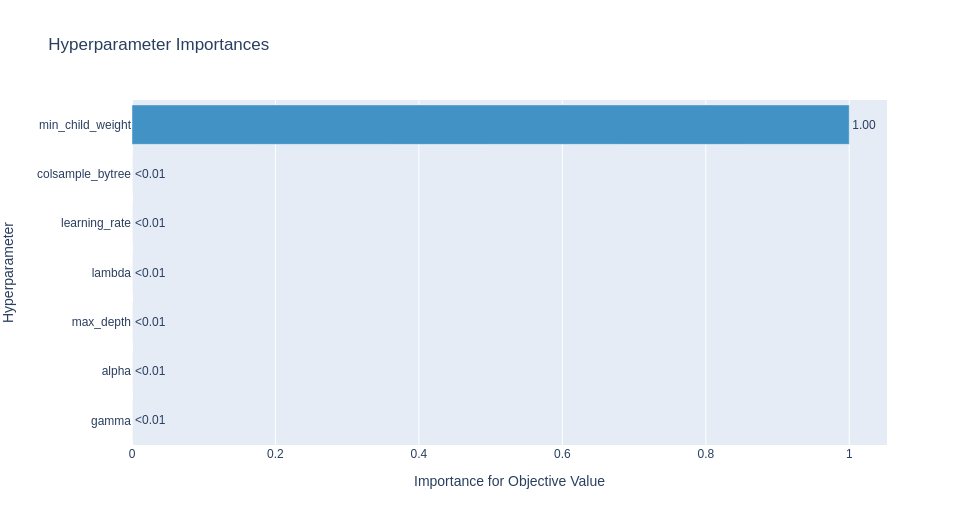
\includegraphics[scale=0.4]{images/optuna_xgboost_imporatnce_cancer.png}
\end{figure}
Ou seja, podemos concluir que ao longo do estudo do Optuna o hiperparâmetro com maior importância no resultado final foi o \textit{min\_child\_weight}.
% \begin{figure}[H]
%  \caption{Hiperparâmetros \textit{min\_child\_weight} do XGBoost no estudo do Optuna no conjunto de dados de Carcinoma de Mama.}.
%  \label{fig:op:cancer:min:xgb}
%  \centering
%  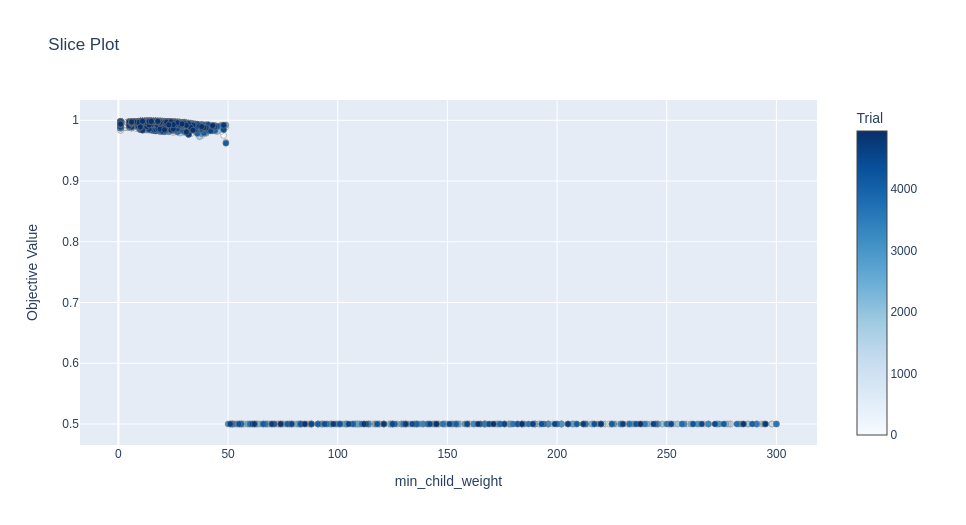
\includegraphics[scale=0.4]{images/optuna_xgboost_min_cancer.png}
% \end{figure}

\subsection{Resultados do estudo do Optuna no conjunto de dados de Carcinoma de Mama utilizando o CatBoost.}
\begin{figure}[H]
 \caption{Valores do estudo do CatBoost no conjunto de dados de Carcinoma de Mama pelo Optuna.}
 \label{fig:op:cancer:trials:cat}
 \centering
 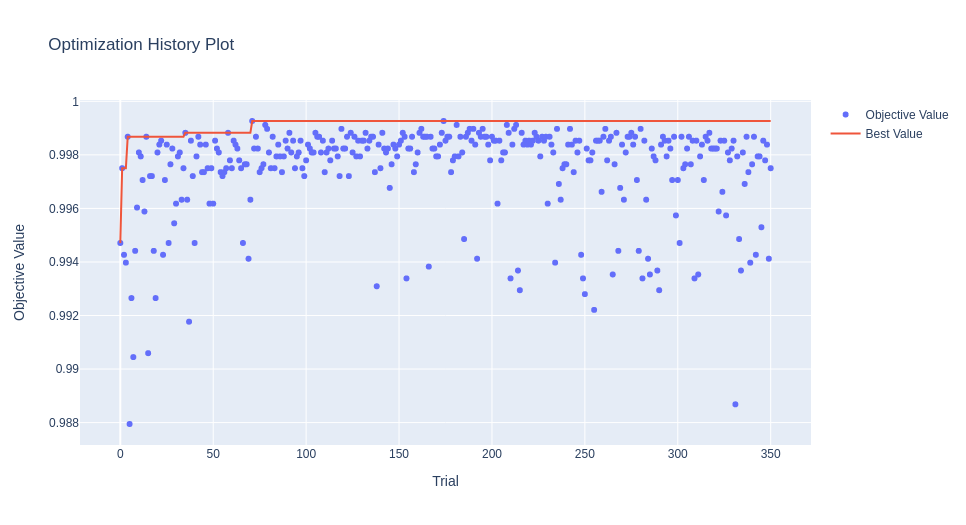
\includegraphics[scale=0.4]{images/optuna_catboost_cancer.png}
\end{figure}
A partir do estudo de otimização do Optuna foi possível identificar quais os hiperparâmetros que possuem o maior impacto no tuning do Optuna.
\begin{figure}[H]
 \caption{Hiperparâmetros do CatBoost com maior importância no Optuna no dados de Carcinoma de Mama.}
 \label{fig:op:cancer:impo:cat}
 \centering
 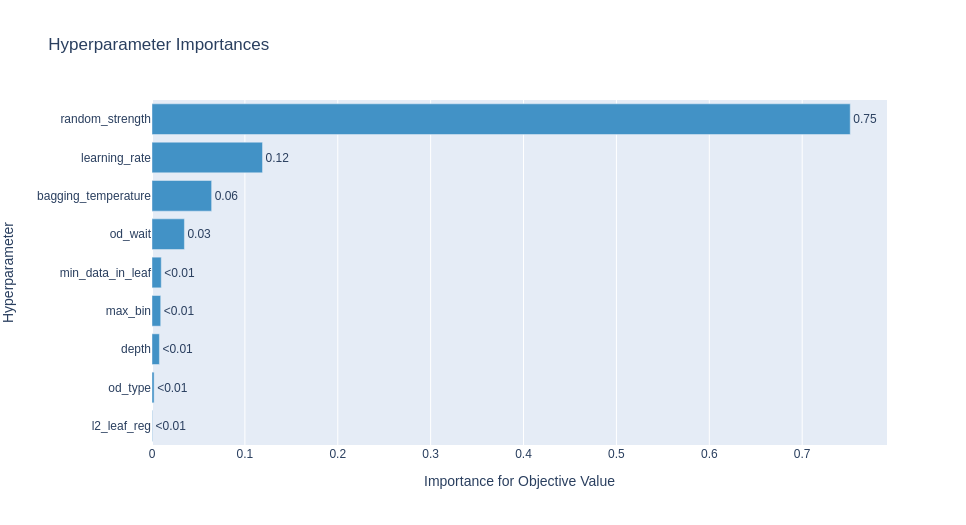
\includegraphics[scale=0.4]{images/optuna_catboost_imporatnce_cancer.png}
\end{figure}
Ou seja, podemos concluir que ao longo do estudo do Optuna o hiperparâmetro com maior importância no resultado final foram o \textit{random\_strength} e o \textit{learning\_rate}.
% \begin{figure}[H]
%  \caption{Hiperparâmetros \textit{random\_strength} do CatBoost no estudo do Optuna no conjunto de dados de Carcinoma de Mama.}
%  \label{fig:op:cancer:rad:cat}
%  \centering
%  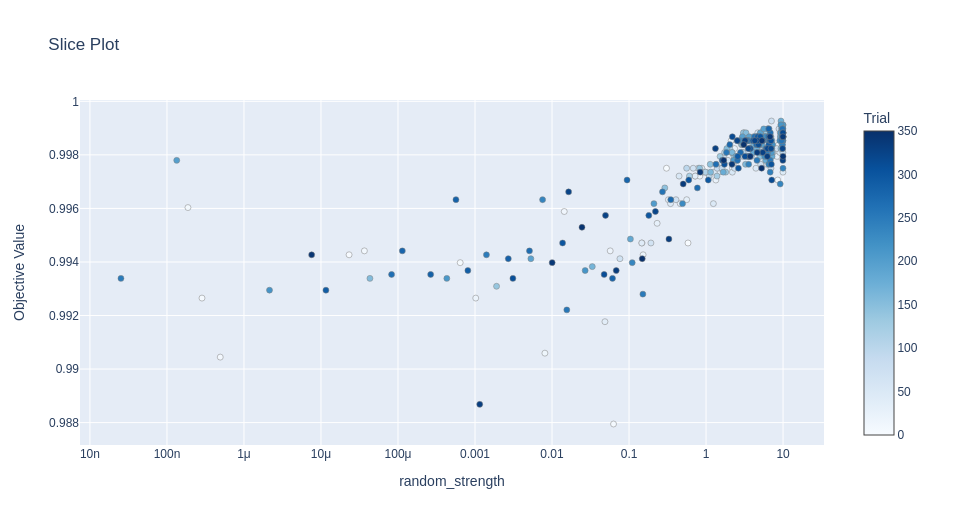
\includegraphics[scale=0.4]{images/optuna_catboost_random_cancer.png}
% \end{figure}
% \begin{figure}[H]
%  \caption{Hiperparâmetros \textit{learning\_rate} do CatBoost no estudo do Optuna no conjunto de dados de Carcinoma de Mama.}
%  \label{fig:op:cancer:len:cat}
%  \centering
%  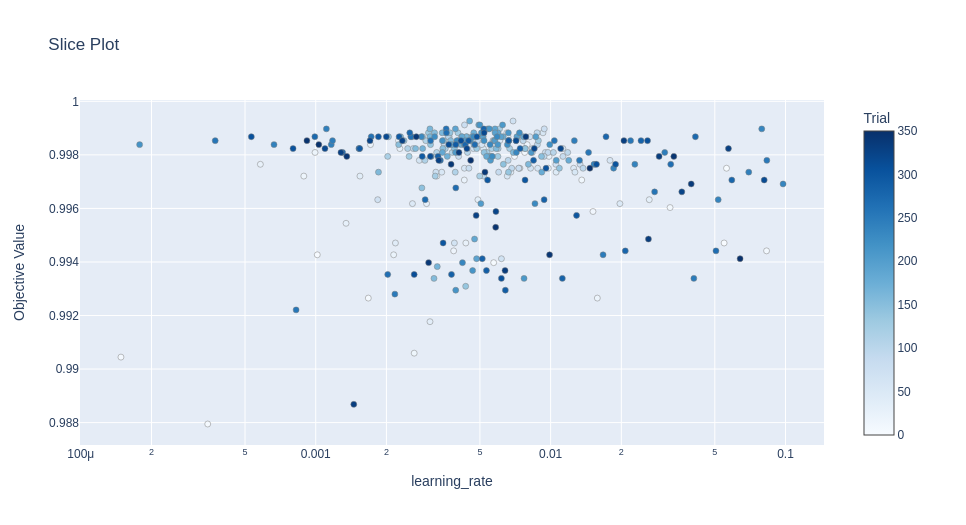
\includegraphics[scale=0.4]{images/optuna_catboost_learning_cancer.png}
% \end{figure}

\subsection{Resultados do estudo do Optuna no conjunto de dados de Carcinoma de Mama utilizando o LightGBM.}
\begin{figure}[H]
 \caption{Valores do estudo do LightGBM no conjunto de dados de Carcinoma de Mama pelo Optuna.}
 \label{fig:op:cancer:trials:lgbm}
 \centering
 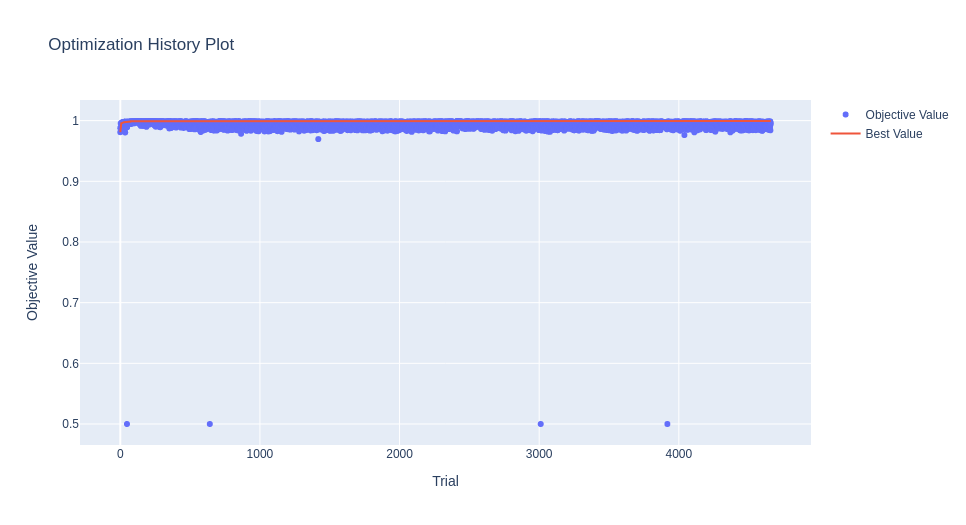
\includegraphics[scale=0.4]{images/optuna_lgbm_cancer.png}
\end{figure}
A partir do estudo de otimização do Optuna foi possível identificar quais os hiperparâmetros que possuem o maior impacto no tuning do Optuna.
\begin{figure}[H]
 \caption{Hiperparâmetros do LightGBM com maior importância no Optuna no dados de Carcinoma de Mama.}
 \label{fig:op:cancer:impo:lgbm}
 \centering
 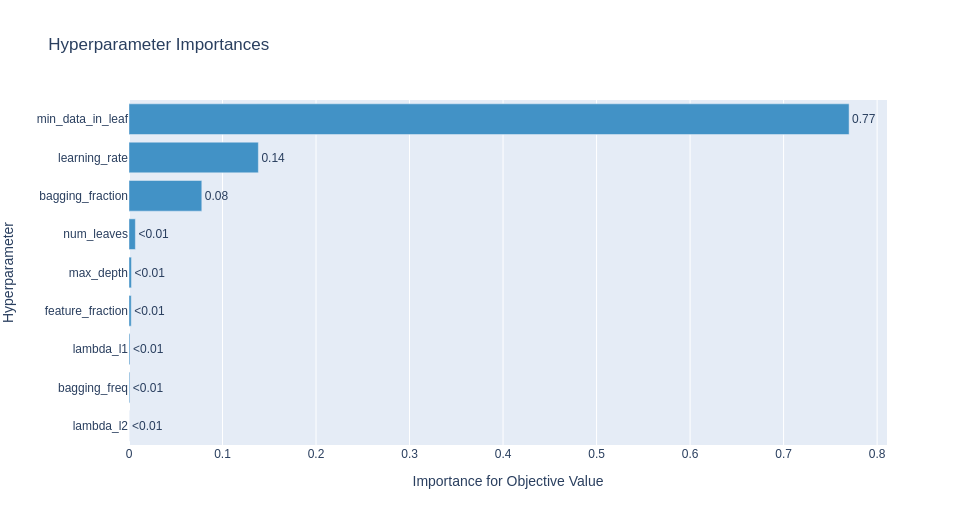
\includegraphics[scale=0.4]{images/optuna_lgbm_importance_cancer.png}
\end{figure}
Ou seja, podemos concluir que ao longo do estudo do Optuna o hiperparâmetro com maior importância no resultado final foram o \textit{min\_data\_in\_leaf} e o \textit{learning\_rate}.
% \begin{figure}[H]
%  \caption{Hiperparâmetros \textit{min\_data\_in\_leaf} do LightGBM no estudo do Optuna no conjunto de dados de Carcinoma de Mama.}
%  \label{fig:op:cancer:min:lgbm}
%  \centering
%  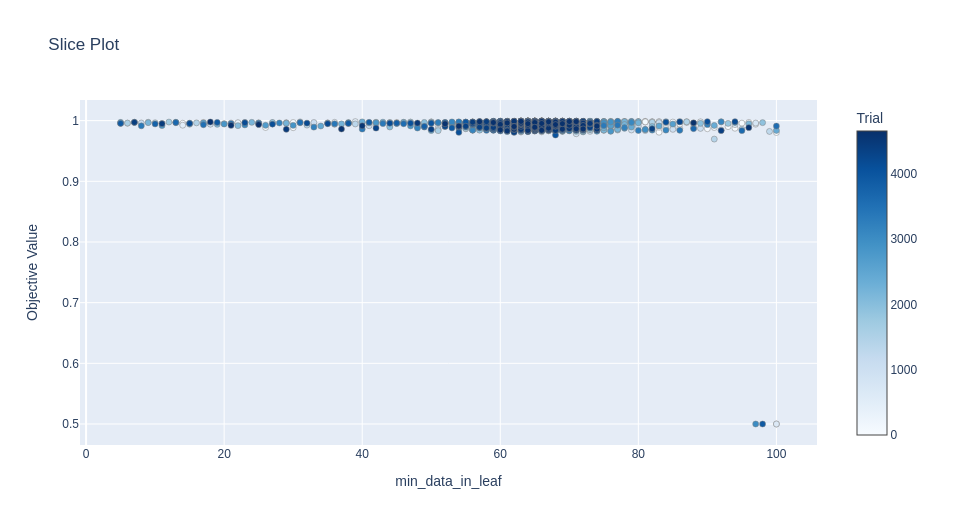
\includegraphics[scale=0.4]{images/optuna_lgbm_min_cancer.png}
% \end{figure}
% \begin{figure}[H]
%  \caption{Hiperparâmetros \textit{learning\_rate} do LightGBM no estudo do Optuna no conjunto de dados de Carcinoma de Mama.}
%  \label{fig:op:cancer:learn:lgbm}
%  \centering
%  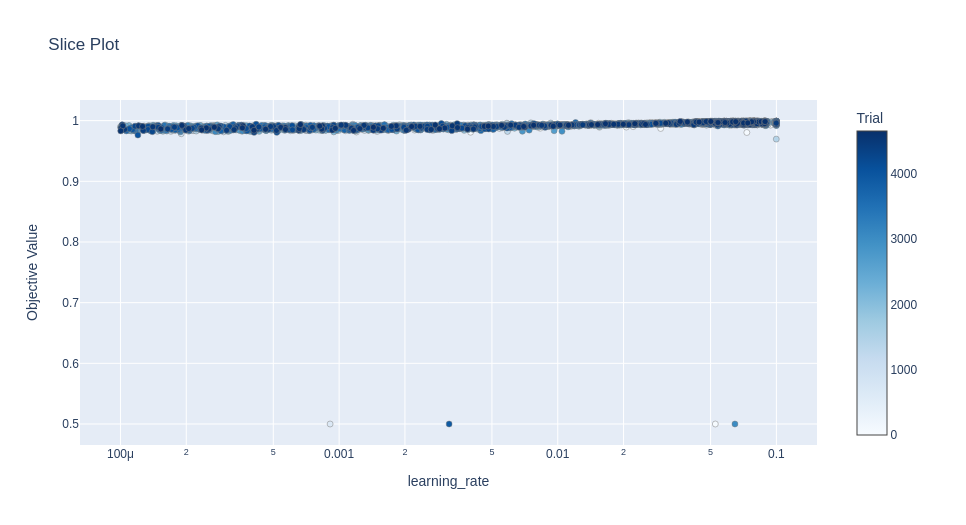
\includegraphics[scale=0.4]{images/optuna_lgbm_learning_cancer.png}
% \end{figure}

